\documentclass[a4paper, twoside, 12pt]{book}

\usepackage[greek, french]{babel}
%--------------------------
% INPUTENC (encodage du texte)
% FONTENC (positionnement des accents)
%--------------------------
\usepackage[utf8]{inputenc}
%\usepackage{ae,lmodern}
\usepackage[T1]{fontenc}

% Interligne
\usepackage{setspace}

%Pour gérer caractères spéciaux °
\DeclareUnicodeCharacter{00B0}{ }
%Pour les épigraphes
\usepackage{epigraph}
\setlength{\epigraphrule}{0pt}
\setlength{\epigraphwidth}{0.6\textwidth}
 \renewcommand\textflush{flushepinormal}
 \renewenvironment{flushepinormal}{}{\vspace*{-\baselineskip}}
\usepackage{booktabs} % Required for better table rules

\usepackage{xltabular}
\usepackage{rotating}
\usepackage{graphicx}
\usepackage{multirow}
\usepackage{longtable}


% Title page details: 
%--------------------------
% HYPERREF (liens hypertextes et métadonnées)
%--------------------------
\usepackage{hyperref}
\usepackage{url}
\hypersetup{%
colorlinks=true,
linkcolor=black,
urlcolor=blue,
citecolor=black
}

\title{Mémoire de Master 2}
\author{Camille Perault}

%--------------------------
% TOCBIBIND (ajouter la bibliographie dans la Table des matières)
%--------------------------
%\usepackage{tocbibind}
\usepackage[nottoc,notlot,notlof]{tocbibind}
%--------------------------
% Éléments de mise en page (marge de 2,5 cm, alinéa en début de paragraphe 1cm, interligne 1,5)
%--------------------------
\usepackage[a4paper, margin=2.5cm]{geometry}
\usepackage{setspace}
\onehalfspacing
\setlength{\parindent}{1cm}

\usepackage{fancyhdr}
\setlength{\headheight}{28pt}
\renewcommand{\chaptermark}[1]{\markboth{#1}{}}
\renewcommand{\sectionmark}[1]{\markright{#1}}
\pagestyle{fancy}
\fancyhf{}
\fancyhead[LE,RO]{\thepage}
\fancyhead[LO]{\nouppercase{\rightmark}}
\fancyhead[RE]{\nouppercase{\leftmark}}
\renewcommand{\headrulewidth}{0pt}

%--------------------------
% Modules pour gérer les listes
%--------------------------
\usepackage{enumerate}
\usepackage{enumitem}


%--------------------------
% BIBLIOGRAPHIE
%--------------------------
\usepackage[backend=biber, sorting=nyt, style=enc]{biblatex}
\usepackage[autostyle]{csquotes}

%\bibliography{mybibliography.bib}
\usepackage{biblatex}
\addbibresource{biblio/agency_language.bib}

\setcounter{secnumdepth}{5}
\setcounter{tocdepth}{2}

\usepackage[official]{eurosym}
\usepackage{afterpage}
\usepackage{booktabs,xltabular}
%--------------------------
% FIGURES
%--------------------------
\usepackage{graphicx}
\graphicspath{ {./images/} }
\usepackage{float}

% ============================================

\begin{document}

\frontmatter
\begin{titlepage}
\begin{center}

\bigskip

\begin{large}
UNIVERSITÉ PARIS, SCIENCES \& LETTRES
\end{large}

\begin{center}\rule{2cm}{0.02cm}\end{center}

\bigskip
\bigskip
\bigskip
\begin{Large}
\textbf{Camille Perault}\\
\end{Large}
\begin{normalsize}
\textit{Diplômée d'HEC Paris}\\
\textit{Diplômée du Master 2 Sciences Cognitives de l'ENS Ulm - PSL}\\
\end{normalsize}

\bigskip
\bigskip
\bigskip

\begin{Huge}
\textbf{DETECTER ET QUANTIFIER L’AGENTIVITE DANS LA LANGUE}\\
\end{Huge}

\bigskip
\bigskip
\begin{LARGE}
\textbf{Une perspective évolutionnaire}\\
\end{LARGE}

\bigskip
\bigskip
\bigskip
\vfill

\begin{large}
Mémoire de deuxième année du master\\
\og Humanités Numériques \fg{} \\
\bigskip
2023
\end{large}

\end{center}
\end{titlepage}

\section*{Résumé}
\addcontentsline{toc}{chapter}{Résumé}
Ce projet interroge la possibilité de détecter de façon cohérente et systématique, dans le langage écrit, une des grandes dimensions psychologiques humaines : celle de l’« agentivité ». En s’intéressant aux ouvrages fictionnels, en particulier les pièces de théâtre pour leur forme stylistique relativement standardisée et leurs personnages types, il entend \textit{in fine} faire le pont entre connotation agentive d’un texte et le degré d’agentivité de son auteur ainsi que de ses contemporains, ce dans une perspective évolutionnaire. Etant donné le caractère très exploratoire de ce travail, et l’ambiguïté de la notion-même d’agentivité étudiée ici, la majeure partie de la recherche a consisté, en amont, à définir plus finement la dimension psychologique en question, et, sur cette base, les marqueurs linguistiques théoriquement à même de refléter le niveau d’agentivité de leurs locuteurs. Ceci explique le relatif déséquilibre entre les chapitres théoriques et ceux ayant trait aux résultats, une grande partie des analyses statistiques restant à mener.


\medskip

\textbf{Mots-clés: agentivité ; psycholinguistique ; anthropologie évolutive ; théâtre classique ; humanités numériques ; lecture distante ; traitement automatique de la langue}

\textbf{Informations bibliographiques:} Camille Perault, \textit{Détecter et quantifier l'agentivité dans la langue : une perspective évolutionnaire}, mémoire de master 2 \og Humanités Numériques\fg{}, dir. [Nicolas Baumard, Jean-Baptiste Camps], Université Paris, Sciences \& Lettres, 2023.


\section*{Abstract}
\addcontentsline{toc}{chapter}{Abstract}
This project investigates the possibility of consistently and systematically detecting, in written language, one of the great human psychological dimensions: that of "agency". By focusing on fictional works, particularly plays for their relatively standardized stylistic form and their typical characters, it ultimately intends to bridge the gap between the agentive connotation of a text and the degree of agency of its author and his or her contemporaries, this in an evolutionary perspective. Given the highly exploratory nature of this work, and the ambiguity of the very notion of agency studied here, the bulk of the research has consisted, upstream, in defining more precisely the psychological dimension in question, and, on this basis, the linguistic markers theoretically capable of reflecting the level of agency of their speakers. This explains the relative imbalance between the theoretical chapters and those dealing with results, with a large proportion of the statistical analyses still to be carried out.

\medskip

\textbf{Keywords: agency ; psycholinguistics ; evolutionary anthropology ; classical theater ; digital humanities ; remote reading ; automatic language processing}

\textbf{Informations bibliographiques:} Camille Perault, \textit{Detecting and quantifying agentivity in language: an evolutionary perspective}, Master 2 thesis \og Digital Humanities\fg{}, dir. [Nicolas Baumard, Jean-Baptiste Camps], Université Paris, Sciences \& Lettres, 2023.


\clearpage
\chapter*{Remerciements}
\addcontentsline{toc}{chapter}{Remerciements}
\markboth{Remerciements}{} 
\bigskip



Je tiens à remercier chaleureusement mon directeur de mémoire Monsieur Nicolas Baumard, pour son enthousiasme pour le projet, sa grande disponibilité, et son aide précieuse tout au long de sa conduite, à commencer par la transmission d’un corpus de théâtre déjà traité qui m’a permise de m’appliquer plus longuement à la définition du cadre théorique.

Je tiens également à remercier Valentin Thouzeau, Edgar Dubourg et Jeanne Bollee, qui ont activement participé à la réflexion autour de ce projet.

J’aimerais enfin remercier Monsieur Jean-Baptiste Camps pour ses conseils et l’intérêt qu’il a su montrer pour ce travail, notamment lors du séminaire de Master.


% table des matières
\addcontentsline{toc}{chapter}{Table des matières}
\tableofcontents

\mainmatter

\part*{Introduction}
\addcontentsline{toc}{part}{Introduction}
\markboth{Introduction}{Introduction}

\vspace*{\fill}
\epigraph{J’entendais tout cela, moi ; car nous autres esclaves, nous sommes doués contre nos maîtres d’une pénétration.}{\textit{Cléanthis, L'île des esclaves, 1725}}

\vfill\clearpage
%abrupt

Au cours du dernier siècle notamment, s’est cristallisée l’idée que l’on assistait à une montée de l'« individualisme », tendance culturelle censée privilégier la valeur et les droits de l'individu par rapport à ceux de la société. De fait, l'individualisme devient dès la seconde moitié du XIX\ieme ~siècle un prisme d’analyse méthodologique à part entière pour la sociologie naissante. De là, le terme semble peu à peu acquérir une connotation négative : il n’est aujourd’hui pas rare qu’il soit apparenté à la dénonciation d’une focalisation excessive sur le soi, un égocentrisme contemporain qui proliférerait au détriment de notre capacité à prêter attention aux autres\footnote{\cite{twenge_generation_2006}}\footnote{\textit{The Century of the Self}, Documentaire BBC : \url{https://www.youtube.com/watch?v=jymMjNc0igI}}.

Or, cette notion portée aux nues par la sociologie-même semble ne pouvoir révéler de manière plus limpide les limites des sciences humaines et sociales « traditionnelles » (du moins dans leur penchant holiste) s’agissant de la compréhension de tels mouvements culturels. Comment, de fait, la tendance à donner la priorité aux individus sur le groupe, contre sa propre cohésion, pourrait-elle s’expliquer en référence à ce même groupe ? Pourquoi le capitalisme, et son pendant psychologique que serait l’individualisme, émergent-t-ils à la fin du XVII\ieme ~siècle ? Et pourquoi pas avant ? Ni plus tard ? Comment, en fond, expliquer un fait social par un autre fait social, pour reprendre l'adage durkheimien, et où s’arrête une telle tautologie ?

Tout d’abord, il faut remarquer que l’on trouve la mention d’idées analogues au concept d’individualisme bien avant l’instauration du système capitaliste, ce dès le Moyen-Âge\footnote{\cite{payen_humanisme_1985}}\footnote{\cite{giddens_modernity_1991}}\footnote{\cite{gourevitch_naissance_1997}}\footnote{\cite{rosenwein_barbara_h_and_c_s_heppleston_y_2005}}. Phénomène non plus spécifiquement moderne, qu’est-ce qui explique, dès lors, que certaines périodes historiques, ou bien encore certaines sociétés, puissent être considérées comme plus individualistes que d’autres ? 

\bigskip

L’anthropologie évolutive s’attache à étudier la diversité des comportements humains dans le contexte de leur histoire évolutive. En particulier, la psychologie « évolutionniste », « évolutive » ou « évolutionnaire », s’intéresse à nos mécanismes de pensée, appréhendés à partir de la théorie de l’évolution biologique. Elle fait de notre environnement et de ses implications pour le fitness de chaque individu, à savoir son succès reproductif, un facteur explicatif central de notre psyché. Sur cette base, elle propose ainsi d’expliquer, ultimement, les modifications des préférences psychologiques humaines qui semblent intervenir au fil de notre Histoire par des variations du niveau de ressources offertes par notre milieu.

Cette précédence périodiquement donnée à l’individu sur le groupe, dans certaines sociétés, pourrait donc être réductible à des considérations matérielles, entendues au sens large (en incluant par exemple l’existence d’institutions). Encore faut-il définir ce qu’est l’individualisme du point de vue de la psychologie individuelle : quel(s) mécanisme(s) de pensée, précisément, pourrai(ent) motiver ces comportements que l’on qualifie synthétiquement d’ « individualistes » ?  Il semble que la notion d’ « agentivité » soit la plus à même de remplir ce rôle. Quoique définie de façon disparate, cette dimension psychologique fait globalement référence à la capacité d’un individu, réelle ou telle qu’elle est perçue par ce dernier, à agir sur le monde qui l’entoure, ce dans le but de poursuivre des objectifs propres. 

En dehors de toute considération hiérarchique, Vallacher\footnote{\cite{vallacher_levels_1989}} développe notamment l’idée que l’on pourrait placer chaque individu le long d’un continuum agentif, selon qu’il envisage le plus souvent ses actions à l’aune de leurs détails mécaniques (faiblement agentif), ou plutôt de significations plus abstraites (hautement agentif).

Pour mesurer un tel degré d’agentivité, l’auteur fait appel au langage : dans son étude, les participants doivent choisir, parmi deux formulations, celle qui décrit le mieux, selon eux, l’activité en question. A titre d’exemple, l’action « nettoyer la maison » (\textit{cleaning the house} en anglais) est alternativement décrite comme le fait de « faire état de sa propre hygiène » (\textit{showing one’s cleanliness}) ou bien simplement de « passer l’aspirateur » (\textit{vaccuming the floor}). Choisir la première formulation est censée dénoter relativement plus d’agentivité qu’opter pour la seconde.

Là où l’auteur ne s’aventure pas, c’est dans la possibilité de systématiser une telle mesure. L’idée que l’utilisation d’un lexique spécifique puisse être corrélée à la possession de certains traits psychologiques n’est pas nouvelle (voir la section I.2.2 \textit{Individualisme et pronoms: même méthode, nouveau raisonnement}), y compris s’agissant d’agentivité. Néanmoins, elle n’a que très rarement été étendue, outre le choix d'un lexique spécifique, à la mobilisation de structures grammaticales ou syntaxiques particulières, qui pourraient s’avérer préférentiellement associées à un état d’esprit plus agentif.

Ce mémoire s’attache donc à déterminer si l’élaboration d’un indice global d’agentivité, construit par agrégation de composantes linguistiques diverses, aussi bien lexicales que « structurelles », est envisageable. Si tel est le cas, l’objectif ultime de cette recherche consistera à mesurer le « score » agentif obtenu par différentes œuvres publiées dans une société donnée au fil du temps, afin de tester l’hypothèse selon laquelle ce score corrèle avec les variations du niveau de ressources de la société en question.

Pour ce faire, nous avons opté pour l’analyse de textes littéraires. Ceux-ci présentaient l’avantage de constituer un corpus conséquent, couvrant une période très large, tout en étant fournis en formules linguistiques suffisamment élaborées. En outre, l’on suppose ici, toujours selon notre paradigme évolutionnaire, que les auteurs de ces œuvres, quoique fictionnelles, se doivent toujours de répondre \textit{a minima} aux attentes de leur public. Ils parleraient ainsi, plus ou moins consciemment, un langage propre à évoquer la psychologie de toute une époque.
\part{Agentivité et langage}

\chapter{Une définition de l’agentivité}
%wrong title 

\section{\textit{The Big Two} : Agentivité et Communion}

Parmi toute la littérature psychologique qui cherche à définir la structure de la personnalité humaine, le modèle des \textit{Big Five} est souvent retenu. Comme son nom l'indique, il s'agit d'un modèle descriptif de la personnalité fondé sur cinq traits centraux (Neuroticisme, Extraversion, Ouverture, Agréabilité et Conscienciosité). Construits par analyse factorielle, ces traits représentent les intercorrélations de comportements spécifiques et répétés, et sont largement supposés constituer les dimensions indépendantes les plus élevées dans la structure hiérarchique de notre personnalité. En d'autres termes, la personnalité d’un individu, entendue ici comme un ensemble de traits comportementaux émis au sein de classes spécifiques définies par leur contenu dans un éventail de situations, et de manière cohérente dans le temps, serait tout au plus réductible à la combinaison de ces cinq traits fondamentaux.

Toutefois, il est apparu récemment que ces facteurs n'étaient pas totalement indépendants, à savoir qu'il existait toujours des corrélations entre certains d’entre eux\footnote{\cite{block_contrarian_1995}}\footnote{\cite{egan_neo-ffi_2000}}. De là ont été définies deux dimensions plus larges encore, qui constitueraient les strates les plus génériques au moment de décrire la structure de notre personnalité, et pour l'instant considérées comme véritablement orthogonales : l’Agentivité et la Communion, communément désignées par le modèle des \textit{Big Two}\footnote{Ces dimensions sont plus ou moins équivalentes aux facteurs Alpha et Beta proposés par {\cite{digman_higher-order_1997}}, et synthétisés chez Wiggins par les métaconcepts d'Agentivité et de Communion (\cite{wiggins_agency_1991})}.

Du latin \textit{agens}, qui signifie « agir » ou « faire quelque chose », l’agentivité est en réalité un concept aux multiples facettes, qui peut revêtir plusieurs significations plus ou moins intriquées. 

Tout d'abord, l’agentivité renvoie à « l'expérience du contrôle de ses propres actions et, à travers elles, des événements du monde extérieur ». C’est ce qu'on appelle plus précisément le « sentiment d’agentivité »\footnote{\cite{haggard_p_chambon_v_sense_nodate}}. En ce sens, l’agentivité est très proche du concept de « locus de contrôle », qui correspond à la croyance qu’un individu entretient sur la relation entre les actions qu’il entreprend et leurs résultats. Cette croyance peut être externe : la personne croit que des facteurs indépendants de sa volonté sont plus importants que ses propres actions au moment de façonner leurs résultats, ou bien interne : il se pense principal maitre à l’œuvre, ce qui correspondrait à un plus grand sentiment d’agentivité.

En relation avec le modèle des \textit{Big Two} cité plus haut, l’agentivité correspond également à « l'une des deux modalités fondamentales de l'existence humaine qui se manifeste dans le contenu de notre perception de nous-mêmes et des autres, dans notre comportement social et dans la manière dont notre personnalité fonctionne »\footnote{\cite{bakan_duality_1966}}. Contrairement à la communion, qui vise à se rapprocher des autres, l’agentivité est centrée sur la poursuite et la réalisation d'objectifs personnels. En ce sens, l’agentivité et la communion peuvent être considérées comme des aspects complémentaires de l'adaptation humaine, qui peuvent interagir pour façonner le comportement social\footnote{\cite{locke_agency_2014}}\footnote{\cite{wiggins_agency_1991}}. Ils répondent en effet à deux besoins fondamentaux en société : le besoin de s'assurer une position sociale avantageuse (ou l’affirmation de soi, étroitement liée à l’agentivité), mais qui doit être modulé avec le besoin d'être intégré dans le groupe (la coopération, soutenue par cette autre dimension psychologique qu’est la communion).

Enfin, l’agentivité peut être comprise comme une relation spécifique entre l'individu et son environnement social, impliquant à la fois un sentiment d’agentivité et une activité réelle, qui se manifeste par la réalisation d'un objectif.

S'appuyant sur cette nature protéiforme qu’il cherche à théoriser, Seligman\footnote{\cite{seligman_m_maymin_p_agency_2022}} considère que l’agentivité est synthétiquement composée de trois éléments : l'efficacité (l'état d'esprit selon lequel on peut atteindre un objectif spécifique maintenant), l'optimisme (l'état d'esprit selon lequel on peut atteindre cet objectif dans un avenir lointain) et l'imagination (l'état d'esprit selon lequel on peut atteindre de nombreux objectifs).

Hitlin et Edler\footnote{\cite{hitlin_time_2007}} ont également proposé une typologie intéressante de l'agentivité, plus directement fondée sur les horizons temporels des acteurs dans les situations d'action, et ses implications pour le soi, comme le détaille le tableau ci-après. Ce modèle nous servira d’heuristique connexe au moment de joindre les approches théoriques de l’agentivité et la psychologie sociale: 

\begin{figure}[!ht]
    \centering
    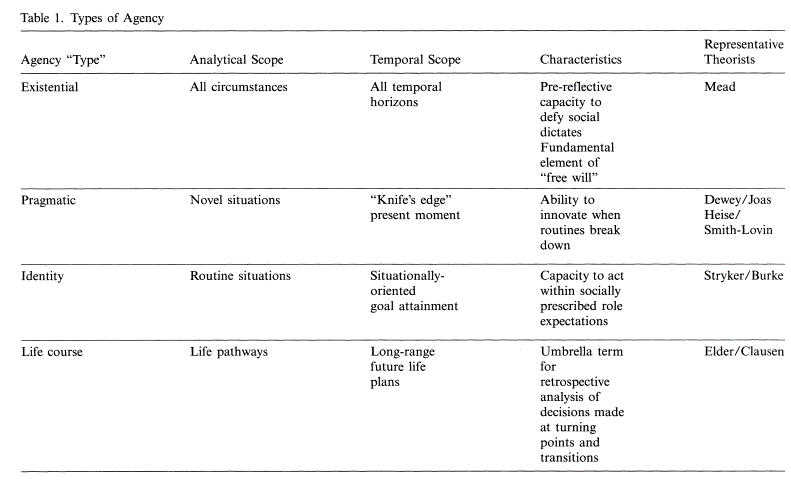
\includegraphics[width=16cm]{img/Types of agency.png}
    \caption{Typologie de l'agentivité s'appuyant sur l'horizon temporel de l'action - Hitlin et Edler (2007)}
    \label{Types_of_agency}
\end{figure}

Ainsi, sous quelque angle que ce soit, l’agentivité implique une activité volontaire et une concentration sur les objectifs de l'individu, qui va de pair avec l’élargissement de son horizon temporel ; et peut être considérée comme une différence individuelle. Plus finement encore, Vallacher\footnote{\cite{vallacher_levels_1989}} intègre la dimension d’agentivité dans sa « théorie de l'identification de l'action », pour en donner une définition qui servira d'inspiration à l'ensemble de ce projet de recherche. Selon lui, étant donné qu'un acte peut être identifié de nombreuses façons par l’individu qui l’exécute, les dispositions comportementales seront inévitablement insuffisantes pour représenter les régularités du comportement, ce qui remet en question la validité même de toute tentative globale de classification des comportements dans des catégories de traits de personnalité \textit{a priori}. Un schéma d'organisation plus raisonnable serait donné par la structure cognitive individuelle des identifications de l’action.

\section{La théorie de l’identification de l’action, ou l’existence d’un continuum agentif}

Pour Vallacher\footnote{\cite{vallacher_levels_1989}}, le niveau d’agentivité personnelle est défini comme « une dimension indépendante qui permet de distinguer à quel point un individu a organisé ses actions en catégories abstraites et significatives qui peuvent servir à canaliser le comportement en tendances dispositionnelles ». En bref, chaque individu pourrait être placé sur un continuum agentif, mesurant son niveau d'identification des actions qu'il entreprend quotidiennement. 

À l'extrémité supérieure du spectre, chez les « agents de haut niveau », la primauté est donnée à la signification de l'action au sens large. Ces agents manipulent des interprétations plus abstraites, distales et centrales de leurs actions, relatives à leurs effets causaux, à la signification véhiculée par la société et à leurs implications à long-terme pour le soi. Les actions sont ainsi dites « orientées vers un but » (\textit{purposed-oriented}). Un tel niveau d’agentivité est associé à une meilleure planification, à une moindre impulsivité et à une plus grande maîtrise de soi\footnote{\cite{fujita_seeing_2008}}, ce quelles que soient les variations contextuelles; ainsi qu’à une représentation plus consciente et plus stable du soi. 

À l'extrémité inférieure du spectre, les agents dits « de bas niveau » se concentrent à l’inverse sur les détails mécaniques de l'action. Ils génèrent des interprétations plus concrètes, locales et périphériques de leurs actions, qui concernent principalement leurs motivations proximales. Ces dernières sont ainsi qualifiées de \textit{means}- ou \textit{process-oriented}, à savoir orientées vers leurs moyens, ou leur processus. Un tel niveau d’agentivité est associé à une préférence pour le court-terme, à un moindre contrôle de soi (plus d'impulsivité, moins d'auto-motivation et moins de cohérence dans le comportement au fil du temps), ainsi qu’à une représentation moins consciente du soi - comme le suggèrent des descriptions de soi moins directement liées aux traits de caractère - et plus volatile, ces individus étant globalement plus sensibles au retour d’information externe\footnote{\cite{fujita_seeing_2008}}.

Une remarque s’impose ici : Vallacher parle « d’identification d’une action » au sens de son interprétation par l'individu, et non d’identification « à » l’action, ou du degré d’investissement identitaire que l'individu engage dans cette même action. Cela étant, les identifications des actions qualifiées de « haut niveau » par Vallacher correspondent de fait à un engagement plus direct de sa propre identité au moment d'interpréter ces dernières, l’action étant notamment appréhendée au regard de ses implications pour la conception de son moi. Nous rapprocherons ainsi directement, dans la suite de cette étude, l’agentivité « haut niveau » à une identification \textit{à} l’action, entre autres facteurs bien sûr.

Par ailleurs, selon Vallacher, « l'identité d'acte particulière qui assume la prépotence pour une personne à un moment donné reflète un compromis entre les préoccupations de compréhension globale [agentivité de haut niveau] et l'exécution efficace de l'action [agentivité de bas niveau] », cette dernière restant la réponse la plus optimale face aux actions nouvelles et/ou complexes, nécessitant une approche plus procédurale pour être exécutées correctement.

A titre d’illustration, un individu peut interpréter son échec à un examen d’abord comme la conséquence d’un manque de chance, du fait d'avoir été confronté à un professeur trop sévère, ou encore d'avoir dû aider ses parents dans une tâche et ainsi de ne pas avoir eu assez de temps pour étudier… ce qui correspondrait à un locus de contrôle externe ou, en nos termes, à une moindre agentivité. Au contraire, il peut s’en rendre directement responsable, en reconnaissant n’avoir pas suffisamment révisé, ce qui témoignerait d’un locus de contrôle interne, ou d’une plus grande agentivité.

Bien entendu, chacune de ces justifications peut être exprimée et détaillée de différentes manières, plus ou moins agentives, et explique qu’on ne réduise pas ici l’agentivité au locus de contrôle, dont la dichotomie constitue la limite. En effet, afin d’expliquer pourquoi il a personnellement failli à un examen, un individu peut alléguer qu’il a simplement fait une impasse sur un chapitre, procrastiné, ou bien qu’il a souvent peur de l’échec et tend ainsi à le prévenir en sapant toutes ses chances de réussite. On sent ici la gradation entre ces différentes réponses en termes d’implication pour le soi, ce bien qu'elles relèvent toutes d’un locus de contrôle interne. De même, en adoptant un locus de contrôle externe, un individu peut simplement affirmer, comme suggéré plus haut, « qu’il n’a pas eu de chance », en notant l’emploi du verbe statif \textit{avoir} qui sera commenté plus tard. Mais il peut également déclarer « qu’il a dû aider ses parents », en utilisant cette fois le verbe modal \textit{devoir}. Là encore, la seconde formulation, bien que toujours déresponsabilisante, semble placer le locuteur dans une posture relativement plus active que le simple fait d'être frappé par la malchance : l’obligation implique en effet, quoique par la négative, un processus de choix, complètement absent de la première interprétation, et dont on pourrait supposer qu’il engage davantage le moi, à savoir la manière dont l’individu se conçoit à partir de cette action (par exemple comme quelqu'un d'excessivement obéissant).

Ce projet consiste donc à tenter de déterminer s’il est possible d’identifier des marqueurs linguistiques fiables permettant d’évaluer, de manière systématique, la teneur agentive d’un texte, et par extension le niveau d’agentivité de son locuteur.

\chapter{Le langage comme reflet de la psychologie humaine}

\section{Transitivité et \textit{foregrounding} : des indices corrélés de l'efficacité de l'action }

Hopper et Thompson\footnote{\cite{hopper_transitivity_1980}} définissent la transitivité comme l'efficacité (\textit{effectiveness}) avec laquelle une action se déroule. Loin de se limiter à la présence d'un Agent et d'un patient, au sens grammatical (un Agent grammatical étant défini comme « une cause unique à partir de laquelle une chaîne ininterrompue de contrôle conduit à l'effet », ou plus simplement comme la responsabilité première d'une entité dans l'effet rapporté sur le monde), elle inclurait les composantes suivantes : 

\begin{figure}[!ht]
    \centering
    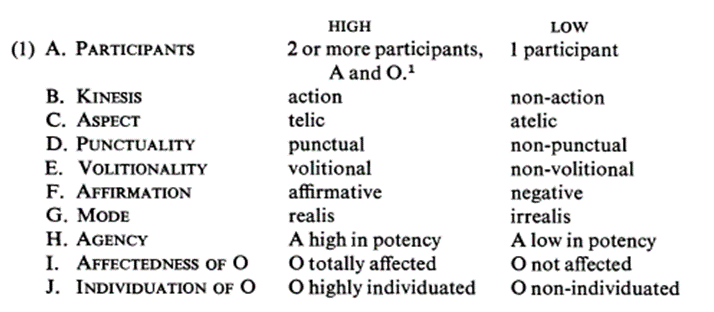
\includegraphics[width=12cm]{img/Hopper_transitivity.png}
    \caption{Elements constitutifs de la transitivité selon Hopper et Thompson (1980)}
    \label{Hopper_transitivity}
\end{figure}

Selon eux, plus une clause a de caractéristiques dans la colonne \textit{haut} (\textit{high}), plus elle est transitive. Ainsi, une phrase avec deux participants comme « Jerry aime la bière », où le patient \textit{bière} ne reçoit pas vraiment d'action, peut en réalité être moins bien notée qu'une phrase avec un seul participant, telle que « Susan est partie ».

Aussi, les auteurs notent que dans toutes les langues examinées au fil de leur étude (qui dépasse largement le cadre de l’anglais, l’approche étant précisément trans-culturelle), les éléments constitutifs de la transitivité covarient largement et systématiquement. Cela signifie qu'à chaque fois qu'une paire obligatoire de deux éléments de transitivité apparait dans la morphosyntaxe ou la sémantique d'une clause, les éléments appariés se trouvent toujours du même côté de l'échelle de la transitivité haute/basse. 

De là, ils considèrent la transitivité comme une propriété centrale de l'utilisation du langage. Probablement en raison d'une limitation psychologique dans le traitement du discours, elle servirait de signal morphosyntaxique des parties du discours qui doivent être stockées pour un traitement séquentiel immédiat (les parties dites « au premier plan » ou \textit{foregrounded}, qui communiquent la structure temporelle du récit), par opposition aux parties qui doivent être stockées pour une référence future ou un accès concomitant (les parties « en arrière-plan », ou \textit{backgrounded}, et qui ne contribuent pas immédiatement ni de manière cruciale à l'objectif du locuteur mais l'assistent, l'amplifient ou le commentent simplement). En bref, la probabilité qu'une clause reçoive une interprétation « de premier plan » est conçue comme proportionnelle à la hauteur de cette clause sur l'échelle de la transitivité. 

Sur la base de cet article, et en prenant le degré d’agentivité du participant comme caractéristique référentielle (ce que les auteurs appellent \textit{potency} ou \textit{agency}), on peut donc postuler que si un participant s’exprime, ou est exprimé, comme ayant plus d’agentivité, toute composante supplémentaire de transitivité présente dans la clause considérée devrait tendre corrélativement vers l'extrémité « haute » de l'échelle. Par exemple, si un événement est évoqué dans une phrase contenant un Agent au sens grammatical, composante linguistique qui semble ainsi la plus directement liée à la notion d’agentivité, cet événement aura tendance à être une action plutôt qu'un état. Et dans le cas particulier d’une action, cette dernière aura tendance à être (interprétée comme) plus volitive et/ou télique, c'est-à-dire représentée comme ayant une fin inhérente, naturelle ou volontaire. Enfin, si un objet est présent avec l'Agent dans une clause donnée, il aura tendance à être plus individué.

Une telle décomposition nous conduit à adopter une approche par faisceau d’indices, en tentant de construire un indice global d'agentivité intégrant toutes ces composantes, et qui devrait être globalement corrélé à l'agentivité du locuteur. L’idée ici est que même si certaines des composantes linguistiques incluses dans l’indice s'avèrent en réalité non corrélées, voire inversement corrélées avec l’agentivité par rapport à nos prédictions, l'indice devrait globalement évoluer dans la même direction que l’agentivité, tandis que des analyses successives pourront permettre de déterminer la qualité et la pertinence de chaque marqueur qui le compose.

Cela étant, la mesure du niveau d’agentivité d’un texte nécessite une modulation des indices proposés par Hopper et Thompson, l’agentivité n'étant plus simplement une composante parmi d'autres de la transitivité mais une variable dépendante à part entière. En ce sens, si l’on considère comme Hopper et Thompson que l'imposition de combinaisons linguistiques particulières dépend fondamentalement de la fonction dominante attribuée au langage, nous pourrions supposer qu’à la place du compromis entre \textit{foregrounding} et \textit{backgrounding} que les auteurs mettent en avant, ou bien au-delà de ce dernier, un compromis s’opère entre un usage purement « communicatif » de la langue et un usage « performatif » (au sens d’un langage conçu d’abord comme vecteur de construction identitaire par le locuteur-même), qui déterminerait l'utilisation préférentielle de constructions morphosyntaxiques potentiellement non chevauchantes, au-delà des seuls marqueurs lexicaux. Une telle conception fait directement écho à l'arbitrage théorisé par Vallacher\footnote{\cite{vallacher_levels_1989}} entre la bonne exécution d'une action (ici, raconter une histoire à quelqu’un) et la compréhension globale de ce qu'elle signifie pour soi (ici, faire du récit lui-même un enjeu identitaire, sujet récurrent en littérature et qui en ferait un champ d'étude privilégié, comme suggéré plus loin dans ce rapport).

Alternativement, si l'on considère que le langage sert toujours d’abord à communiquer, en retenant donc le fondement psychologique proposé par Hopper et Thompson, il est possible d'envisager qu’un langage plus agentif corresponde à un autre type de \textit{foregrounding} que celui mentionné par les auteurs, motivé par cette dimension psychologique spécifique qu’est l’agentivité. Plutôt que sa structure temporelle, le locuteur s’attacherait alors à mettre en avant la structure identitaire de son récit, ce qu'il dit sur son \textit{soi}. Là encore, ce \textit{foregrounding} pourrait impliquer des composantes linguistiques spécifiques, ne correspondant pas totalement à celles qui participent de la transitivité, ou efficacité temporelle, d’un discours. Néanmoins, l’on s’attendrait à trouver un certain nombre de convergences linguistiques entre ces deux motifs, l’agentivité étant crucialement dépendante de la capacité à adopter une perspective plus long-termiste, tel que le suggérait le modèle de Hitlin et Edler précédemment cité et les différentes manières de considérer le soi en fonction du cadre temporel adopté. Le soi peut en effet être considéré comme un instrument conceptuel nécessaire, un liant sémantique dont la fonction originelle serait précisément de permettre la pensée exploratoire\footnote{\cite{hills_foraging_2015}}, c'est-à-dire d'être orienté vers le futur, et ainsi de s’autoréguler à plus long terme par la rétrospection et l'anticipation, plutôt que de moduler sa performance dans le présent, focalisation caractéristique d’individus peu agentifs.

Si l’agentivité au sens grammatical (\textit{potency} ou \textit{agency}) du participant, sa volitionnalité et l’aspect télique de la clause en question, participant de sa transitivité selon Hopper et Thompson, peuvent également être considérés comme dénotant de manière concordante un degré supérieur d’agentivité, au sens de Vallacher, cela est cependant moins évident s'agissant de l'individuation de l'objet grammatical, définie par Hopper et Thompson de la manière suivante :

\begin{figure}[!ht]
    \centering
    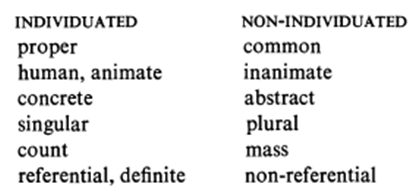
\includegraphics[width=8cm]{img/Hopper_individuation.png}
    \caption{Eléments participant de l'individuation de l'objet grammatical selon Hopper et Thompson (1980)}
    \label{Hopper_individuation}
\end{figure}

De fait, bien qu'elle soit considérée comme une composante transitive « faible » dans le tableau ci-dessus, nous nous attendons plutôt à ce que l'abstraction soit corrélée avec un niveau supérieur d’agentivité, étant donnée l’interprétation plus conceptuelle de leurs actions qui caractérise les agents « haut niveau ». Il en va de même pour les modes de l’irréel, classés par les auteurs dans la partie « basse » de l’échelle transitive. 

La direction de la corrélation, si elle existe, pour la composante d'affirmation n'est quant à elle pas évidente s’agissant d’agentivité. Cela peut s'expliquer par le fait qu’Hopper et Thompson définissent la transitivité comme l'\textit{efficacité} d'une action, à savoir son caractère plus ou moins réalisé, là où l’agentivité inclut également, pour reprendre la tripartition de Seligman\footnote{\cite{seligman_psychological_2023}}\footnote{\cite{seligman_psychological_2023}}, l'optimisme et l'imagination, que nous subsumerons sous la notion de « capacité de distanciation psychologique », ainsi que « l'auto-efficacité » ou « sentiment d’agentivité », qui n’est que partiellement corrélé à l’efficacité des actions entreprises par l’individu.

\section{Individualisme et pronoms : même méthode, nouveau raisonnement}

Le langage a souvent été utilisé comme un indicateur de dimensions psychologiques ou traits de personnalité spécifiques, ce à différents niveaux d'analyse. L'utilisation des pronoms en particulier, et leur lien avec la notion d'individualisme, a fait l'objet de nombreuses études. Nous précisons que toutes ces études traitent de l’anglais, et non du français. Néanmoins, et malgré l’existence de différences certes importantes entre ces deux langues, il semble n’y avoir aucune raison de penser qu'une approche psycholinguistique ne puisse s’appliquer au français également, et qu’elle révèlerait qui plus est les mêmes associations que celles décrites ci-après, étant donnés les marqueurs linguistiques relativement simples considérés ici, ainsi que les similitudes culturelles entre ces deux pays. 

Dans une étude de 1998, Kashima et Kashima\footnote{\cite{kashima_culture_1998}} ont constaté que l'augmentation de la richesse et le changement climatique prédisaient l'individualisme, mais que le résultat était modulé par l'utilisation de la langue : les cultures individualistes auraient tendance à favoriser l'utilisation explicite des pronoms de la première personne, tandis que les cultures collectivistes permettraient aux locuteurs d'abandonner les pronoms de la première personne dans la structure superficielle des phrases\footnote{Voir également \cite{yu_cultural_2016}}. De manière cohérente, l'utilisation de langues spécifiques, comme l'anglais, a été associée à des concepts de soi plus indépendants chez les personnes bilingues\footnote{\cite{marian_self-construal_2004}}. Plus généralement, des recherches antérieures ont établi un lien entre les pronoms de la première personne du singulier (tels que « je », « moi ») et l'individualisme d'une part, et entre les pronoms de la première personne du pluriel (tels que « nous ») et le collectivisme d'autre part\footnote{\cite{gardner_i_1999}}\footnote{\cite{kashima_culture_1998}}\footnote{\cite{na_culture_2009}}.  

Au sein d’une même culture, Twenge\footnote{\cite{twenge_changes_2013}} a pu observer que, dans les livres américains publiés entre 1960 et 2008, l'utilisation des pronoms de la première personne du pluriel avait diminué de 10\%, tandis que les pronoms de la première personne du singulier avaient augmenté de 42\%, et les pronoms de la deuxième personne (« tu », « toi ») quadruplé. Cela suggérerait d'après l'auteure la montée d'un individualisme aux Etats-Unis, avec une tendance parallèle vers moins de collectivisme.

Ces résultats peuvent être examinés à la lumière des recherches sur l'utilisation individuelle des pronoms : dans la correspondance personnelle et le discours, les pronoms singuliers de la première personne ont également été associés à une plus grande focalisation sur l'individu, ainsi qu'à un statut inférieur, à l'honnêteté, à la dépression et à un style plus personnel et plus expressif. A l’inverse, les personnes de statut supérieur utiliseraient davantage de pronoms de la première personne du pluriel et de la deuxième personne\footnote{\cite{nerbonne_secret_2014}}.

Si l’on tente de faire dialoguer ces deux niveaux d’analyse, culturel et individuel, les résultats de Twenge suggèrent donc que le langage (américain) aurait « évolué pour devenir moins hiérarchique, plus centré sur soi et plus expressif (peut-être dépressif) », bien que cela ne soit en accord qu'avec certains éléments de l'individualisme seulement (augmentation de l'expression émotionnelle, moins de hiérarchie dans l'ensemble, plus d'égocentrisme), mais pas nécessairement avec d'autres (plus d'excès de confiance et de revendication de statut, ce qui contraste avec l'association, au niveau individuel, entre un statut inférieur, l'honnêteté et la dépression d'une part, et l'utilisation de pronoms à la première personne du singulier d'autre part). L'utilisation de la deuxième personne en particulier, est associée à un statut supérieur et augmenterait avec le temps, de sorte que les résultats en matière de statut sont au mieux décrits comme mixtes.

Dans le même ordre d'idées, une analyse linguistique des 10 chansons américaines les plus populaires entre 1980 et 2007\footnote{\cite{dewall_tuning_2011}} a mis en évidence des changements dans l'utilisation de mots censés refléter des changements psychologiques : au fil du temps, l'utilisation de mots liés à la focalisation sur soi et au comportement antisocial aurait augmenté, tandis que les mots liés à la focalisation sur l'autre, aux interactions sociales et à l'émotion positive semblent avoir diminué.

Enfin, Twenge\footnote{\cite{twenge_generational_2012}} a constaté que, par rapport aux générations précédentes, un plus grand nombre d'étudiants américains se considèrent aujourd'hui comme « supérieurs à la moyenne » s'agissant d'attributs tels que les capacités académiques, la volonté de réussir, les capacités de leadership, la capacité à s'exprimer en public, la confiance en soi et la capacité à écrire (ce en tenant compte de la race, du sexe, des performances et du temps passé à étudier, ce dernier étant en fait en baisse ; et en dépit du fait que la population universitaire soit devenue moins sélective). L'auteure conclut que de vastes changements culturels mettant l'accent sur une vision positive de soi (aux États-Unis du moins) ont apparemment entraîné une amélioration des auto-évaluations dans les domaines agentifs, tandis que les auto-évaluations des attributs communautaires, tels que la compréhension des autres, la coopération et la spiritualité, auraient soit diminué, soit stagné. Aussi, les produits culturels, notamment dans leur forme linguistique, fonctionneraient à leur tour pour entretenir et accélérer de tels changements générationnels, vers la démonstration de traits psychologiques de plus en plus individualistes (en incluant dans cette notion aussi bien l'estime de soi, l’agentivité et le narcissisme).

Cependant, l'ambivalence du lien entre l'individualisme au niveau culturel et individuel mentionnée plus haut pose question, et pourrait laisser penser que l’agentivité est ici définie de manière trop restrictive. En effet, Twenge semble assimiler l’agentivité à un trait de personnalité parmi d'autres, qui résulterait de l'intériorisation d'un individualisme croissant au niveau culturel, les deux se renforçant alors mutuellement. En outre, cet individualisme est compris comme une valeur culturelle donnant la priorité à l'individu sur la collectivité, et est donc étroitement lié à l'affirmation de son propre statut dans le monde, vécu positivement. Non seulement ce raisonnement ne s'inscrit pas dans une approche évolutionnaire que nous expliciterons ci-après, mais nous adoptons une définition plus globale de l’agentivité personnelle, qui ne se résume pas à un jugement positif sur ses propres capacités individuelles, ou estime de soi. Twenge elle-même semble y faire allusion lorsqu'elle considère que ces auto-évaluations plus mélioratives des étudiants américains pourraient résulter, plutôt que d'un égocentrisme plus prononcé, du fait que «les étudiants récents interprètent les attributs de manière plus large que les générations précédentes, trouvant plus de façons de se considérer comme supérieurs à la moyenne »\footnote{\cite{dunning_ambiguity_1989}}. Cette « surinterprétation » correspondrait, en nos termes, à un niveau d’agentivité plus élevé, dans la mesure où un individu qui tend à identifier ses actions de manière plus abstraite au quotidien pourrait être corrélativement plus désireux et/ou capable d'extrapoler n'importe quelle notion, au-delà des actions seules, et d'en trouver ainsi une certaine définition selon laquelle on pourra dire qu'il est particulièrement performant - ce d’autant plus s’il s'agit de compétences métacognitives alors \textit{de facto} plus développées.

Si l'on peut s'attendre à ce qu'un niveau d'agentivité plus élevé favorise l'apparition de certains traits individualistes (narcissisme, extraversion, etc.), il n'y a donc pas de raison de postuler une correspondance biunivoque entre les deux concepts. La tendance au neuroticisme, par exemple, pourrait précisément être associée à un « débordement » de l'agentivité « haut niveau », ce contrairement à ce que l'individualisme appréhendé au niveau culturel semble prédire. Dans ce cas, l'individu serait incapable de passer à un niveau de conceptualisation engageant relativement moins son moi dans des situations nouvelles et/ou complexes, et serait donc amené à s’investir outre-mesure dans ce qui risque d'être mal exécuté, menaçant ainsi l'image de soi (comme le reflète le langage utilisé dans les communications personnelles).

Selon cette logique, il est alors possible de dépasser la conception péjorative de l'individualisme, définie comme un simple égocentrisme, pour le comprendre plutôt comme le corollaire naturel d'une plus grande agentivité, dont on rappelle l’orthogonalité supposée avec la communion.

\part{Questions de recherche et méthodologie}

\chapter{L’évolution de nos préférences psychologiques, un paradigme évolutionnaire}

\section{Les fondements de la psychologie évolutive}

Comme pressenti plus haut, le pouvoir explicatif des grands mouvements culturels appliqués aux changements dans la psychologie et le comportement des individus peut paraitre assez limité. En l’occurrence, l'idée qu'avec la montée de l'individualisme, appréhendé comme une évolution culturelle \textit{sui generis}, chaque individu aurait tendance à devenir de plus en plus égocentrique, contribuant ainsi à enraciner l'avènement de cette nouvelle ère du « je » au niveau collectif (qui n’existe en réalité que par la somme de ses membres) frustre par son apparente circularité.

Le paradigme évolutionnaire constitue ainsi une explication alternative intéressante, où l'Histoire est bien celle des individus avant d’être celle du groupe. Selon lui, notre plasticité adaptative, définie comme la capacité à moduler notre phénotype (à savoir l'ensemble de nos caractéristiques observables) en fonction de l'environnement, impliquerait notamment la modulation de nos préférences psychologiques. Ces changements psychologiques seraient les mécanismes « proximaux » permettant \textit{in fine} à chaque individu d'optimiser sa stratégie d'allocation des ressources en fonction des transformations de son milieu (cette stratégie constituant le mécanisme « ultime » dans l'optimisation de son succès reproductif individuel).

Car le phénotype optimal d'un individu, qui inclut, outre ses caractères physiques, ses stratégies comportementales, traits de personnalité et préférences psychologiques, varie de fait en fonction des ressources disponibles dans son environnement, entendues au sens large (matérielles, institutionnelles, etc). En particulier, les modèles d'allocation optimale des ressources montrent que les individus devraient investir dans les besoins dont le rendement marginal est le plus élevé. Et étant donné que les besoins ont des rendements marginaux décroissants, lorsque les individus ont plus de ressources à investir, ils commenceraient à allouer des ressources à de nouveaux besoins. A mesure que les individus progressent dans la pyramide des besoins\footnote{\cite{maslow_theory_1943}}, leur psychologie se modifierait, et ils développeraint des préférences leur permettant, ultimement, de tendre vers la satisfaction des besoins devenus les plus adaptatifs dans l'environnement considéré (à savoir ceux qui maximisent leur \textit{fitness}, qui constitue la représentation quantitative du succès reproductif de l'individu).

\begin{figure}[!ht]
    \centering
    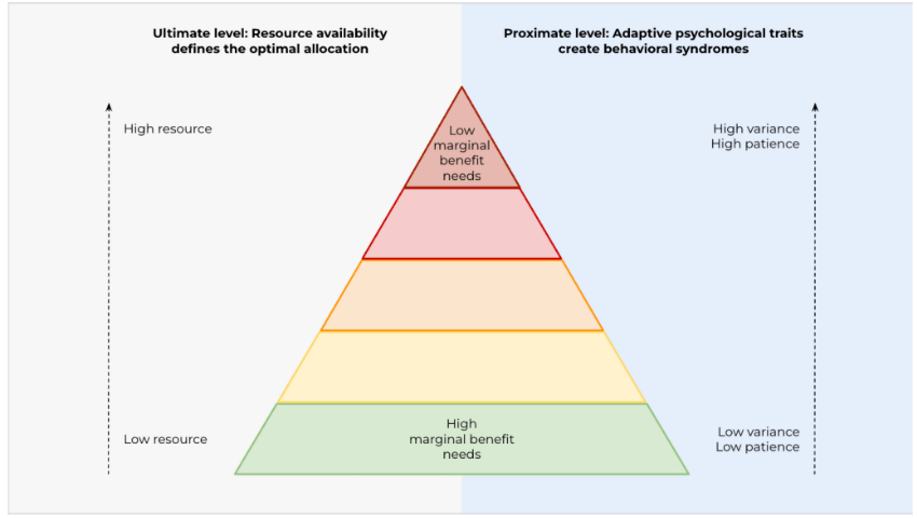
\includegraphics[width=17cm]{img/pyramide_besoins.png}
    \caption{La Pyramide des besoins de Maslow (1943) intégrée à un paradigme évolutionnaire}
    \label{pyramide_besoins}
\end{figure}

À cet égard, et en ce qui concerne l'agentivité, au fur et à mesure que l'environnement devient plus riche et plus prévisible, il deviendrait de plus en plus adaptatif pour un individu de se penser comme capable d'avoir une prise sur le monde extérieur, précisément parce que l'autonomie devient alors possible, et que les efforts investis sont susceptibles de générer des bénéfices individuels additionnels. A l'inverse, dans un environnement très incertain et/ou hostile, il serait plus adaptatif de se sentir relativement moins agentif et de préférer s'en remettre à l'apprentissage de lois extérieures alors perçues comme « naturelles ». Cela permettrait en effet de s'en accommoder au mieux, puisqu'il serait \textit{de facto} plus difficile, voire impossible, d’infléchir ces forces extérieures en faveur de projets autonomes, ces derniers représentant alors un effort relativement vain, voire désavantageux en termes de fitness.

Autant de considérations qui font écho au compromis de Vallacher\footnote{\cite{vallacher_levels_1989}} mentionné précédemment, mais formulé cette fois en des termes évolutionnaires : lorsque la quantité de ressources dans l'environnement est suffisamment élevée pour que la plupart des actions réalisées soient relativement faciles à prendre en charge (y compris la possibilité de s'appuyer sur un système institutionnel pour déléguer une partie de la satisfaction de ses besoins « les plus bas »), l'individu n'aurait plus besoin de s'attarder sur leurs détails mécaniques, et pourrait se permettre d'allouer ses ressources cognitives à l’interprétation plus abstraite de ses actions, le développement de capacités de planification associées étant susceptible d'optimiser son succès reproductif à plus long terme. 

De tout ce qui précède, deux questions de recherche se posent pour nous, dont seule la première sera abordée dans le cadre de ce mémoire : 

1. Est-il possible de construire un indice linguistique d'agentivité, c'est-à-dire un faisceau de marqueurs linguistiques qui permette de mesurer le degré d'agentivité d'un texte, et par extension, de son locuteur ?

2. Si tel est le cas, comment l’agentivité, mesurée par un tel indice, varie-t-elle avec le temps et les ressources dans une société donnée ? Sur la base du paradigme adopté, nous supposons que le niveau « moyen » d’agentivité dans une société devrait être positivement corrélé avec son niveau de ressources.

\section{Les fictions narratives, des « produits dérivés » de l’esprit humain}

Si notre ambition ultime est celle d’exploiter notre indice linguistique pour retracer l’évolution de l’agentivité d’individus réels, pourquoi donc l’élaborer à partir de textes fictionnels ? Il se trouve que notre paradigme évolutionnaire fait de la fiction narrative un support particulièrement pertinent pour retracer l'histoire de la psychologie humaine. 

De fait, il est possible de considérer les fictions narratives comme des « produits dérivés » de l'esprit humain, à savoir qu'elles n'auraient pas évolué par sélection naturelle mais auraient coopté certaines préférences et mécanismes cognitifs préexistants, sélectionnés avant même l'émergence de la culture symbolique et pour d'autres raisons liées à notre Environnement d'Adaptation Évolutive (l'environnement ancestral auquel notre espèce est adaptée)\footnote{\cite{dubourg_why_2022}}. Selon cette hypothèse, la fiction survit car nous tirons certains bénéfices de la production et de la consommation de ces objets culturels attrayants, ce qui la rend indirectement adaptative.

Les fictions narratives peuvent ainsi être considérées comme des « technologies de divertissement », à savoir comme des objets conçus par certaines personnes dans le but immédiat d'attirer l'attention des autres, et dans le but ultime de remplir d'autres fonctions évolutives pertinentes qui deviennent plus faciles à atteindre une fois que l'attention des autres a été captée. Cela permettrait d'expliquer pourquoi la fiction est souvent remplie de stimuli exagérés et divertissants, pourquoi elle s'adapte si bien aux préférences changeantes du public qu'elle cible, et pourquoi les producteurs rendent leur fiction de plus en plus attrayante au fil du temps, ce de manière cumulative.

Les fictions peuvent donc servir de miroir pour retracer l'évolution dans le temps de ces préférences psychologiques que chaque lecteur dicte et que chaque auteur coopte, et qui changent en fonction des transformations du milieu.

\chapter{Construction d’un indice d’agentivité global : une approche par faisceau d’indices}

\section{Validation interne : le choix d’un corpus théâtral}

Se pose alors la question du corpus à sélectionner pour éprouver notre indice agentif, dont nous détaillerons la composition dans la partie suivante. Les indicateurs linguistiques ayant été choisis sur la base de la langue française, l'étude porte ici sur les productions littéraires françaises.

En particulier, la forme stylistique relativement standardisée du théâtre permet de contrôler certaines variations qui pourraient être liées à des phénomènes plus aléatoires de transmission culturelle plutôt qu'à la sélection et à la plasticité proprement dites, qui font du passage d'une préférence psychologique à une autre la réponse spécifique et optimale à certains changements environnementaux, préférence qui se refléterait en partie dans le choix des mots.

Le genre théâtral présente également l'avantage de disposer de corpus substantiels déjà constitués et librement accessibles en ligne. En l'occurrence, nous avons choisi de retenir le corpus de théâtre classique librement téléchargeable sur le site \small{\url{www.theatre-classique.fr}}, comprenant les principales œuvres théâtrales publiées en France entre 1550 et 1800.

Surtout, la dualité théâtrale classique entre personnages maîtres et serviteurs fournit un critère de validation interne particulièrement solide pour notre indice agentif. Par définition, il semble en effet raisonnable de considérer que les maîtres sont relativement plus agentifs que leurs serviteurs. Il s’agira alors de comparer le score global de l'indice obtenu pour les répliques prononcées par tous les personnages maitres et serviteurs respectivement, une première étape pour tester la capacité de l’indice à tracer \textit{quelque chose comme l'agentivité} dans un texte.

Concrètement, nous avons attribué à chaque personnage des pièces étudiées un statut sur la base des mots-clés apparaissant ou non pour le décrire dans la didascalie de chaque pièce. Pour considérer un personnage comme « serviteur », ou plutôt comme doté d’un « bas statut » (le terme de « serviteur » est entendu ici dans un sens générique), statut pour lequel les mentions dans la didascalie étaient les moins ambiguës, nous avons retenu les mots-clés suivants : « domestique », « esclave », « chambre » (pour « femme de chambre »), « camariste », « servant », « servante », « suivante », « valet », « suite », « confident », « confidente ». Notons que nous avions accès à une liste de tous les « rôles » pris par les personnages dans l'ensemble du corpus, référencée par le site mentionné ci-dessus. C'est à partir de cette liste que nous avons construit notre liste de mots-clés, qui se trouve donc être exhaustive pour ce corpus.

Pour les personnages dits « haut statut », dont les mentions étaient parfois ambiguës ou simplement trop variées pour procéder par liste de mots-clés malgré l'existence d'un tel référencement, nous avons retenu la règle suivante : tout personnage dont le nom X apparaît en complément d'un mot-clé « bas statut » (par exemple « valet de X ») est automatiquement considéré comme appartenant au groupe « haut statut », dans le sens où il a quelqu'un à son service. Cela semblait être la manière la plus neutre et la plus pertinente de procéder, sans être soumis aux variations socio-historiques dont pourrait souffrir le sens d'étiquettes telles que « bourgeois », et en relation avec notre concept d'agentivité - l'idée étant qu'un personnage capable d'en commander un autre est \textit{a fortiori} plus agentif que celui qu'il ou elle commande. Pour chaque pièce considérée, les répliques des personnages qui ne répondaient pas à ces critères dans la didascalie, et n’appartenaient donc à aucun des deux groupes, ont été exclues de l'analyse linguistique.

A partir de là, nous avons codé une manière d'attribuer à chaque personnage inclus dans l’analyse les répliques qu'il ou elle formulait dans l'ensemble de la pièce. Nous avons ensuite concaténé l’ensemble des répliques respectivement prononcées par des personnages « bas » et « haut » statut, afin de pouvoir comparer leur score agentif au niveau de chaque pièce.

\section{Validation externe : plusieurs propositions}

Nous avions également besoin d’une validation externe de notre indice, afin de s’assurer qu’il trace l’agentivité spécifiquement, sans être corrélé à d'autres dimensions psychologiques telles que la communion, auquel cas il ne saurait être informatif.

À cette fin, il existe tout d’abord une vaste littérature établissant un lien entre agentivité et masculinité\footnote{\cite{neria_encyclopedia_2016}}. Examiner en parallèle si l'indice est préférentiellement corrélé avec les répliques de personnages masculins plutôt que féminins était ainsi une première façon de s'assurer de la spécificité de sa mesure.

En outre, il nous a semblé utile de comparer notre indice avec des marqueurs linguistiques spécifiques d’autres dimensions psychologiques, pour lesquelles nous ne nous attendions pas à des corrélations avec le statut du personnage, et par conséquent avec l'indice agentif. Malheureusement, aucune étude à ce jour ne s'est intéressée aux corrélations potentielles entre la communion, \textit{a priori} orthogonale à l’agentivité, et certains marqueurs linguistiques, ce qui suffirait à faire l'objet d'un projet de recherche à part entière. 

Il a donc fallu se tourner à nouveau vers le modèle des \textit{Big 5}, en dépit de ses limites. Il se trouve en effet que certains des cinq traits qui le composent entretiennent une relation privilégiée avec les deux dimensions supérieures que sont l’agentivité et la communion. 

Pour l'observer, il faut en réalité mobiliser, outre les modèles dimensionnels comme celui des \textit{Big Five}, la notion de circomplexes. Egalement très utilisés en psychologie pour décrire les relations entre un ensemble de variables, les modèles circomplexes sont généralement définis en termes de corrélations systématiques croissantes et décroissantes entre les variables, et peuvent être représentés visuellement sous la forme d'un cercle dans lequel les variables adjacentes sont fortement corrélées et les variables opposées sont inversement corrélées. Ils ont notamment été utilisés pour décrire les dispositions interpersonnelles\footnote{\cite{wiggins 1979}}. 

A partir d’un échantillon de 315 hommes et femmes adultes, et en factorisant conjointement les auto-évaluations passées sur les Échelles d'Adjectivité Interpersonnelle révisées de Wiggins\footnote{Le comportement interpersonnel ayant souvent été caractérisé par des modèles circumplexes, Wiggins a entrepris de créer un ensemble d'échelles adjectives présentant des propriétés circumplexes, et auxquelles on se réfère ici. Voir \cite{wiggins_psychological_1979}} avec des auto-évaluations, des évaluations par les pairs et des évaluations par le conjoint fondées sur l'Inventaire de Personnalité NEO\footnote{Le NEO-PI est un questionnaire de 181 items développé pour opérationnaliser le modèle à cinq facteurs. Les réponses aux items du NEO-PI se font sur une échelle de Likert en 5 points. Une forme à la troisième personne du NEO-PI a également été mise au point et validée pour être utilisée par des évaluateurs. \cite{costa 1985}}, ce afin d'examiner les relations entre les deux modèles, McCrae et Costa\cite{mccrae_structure_1989} ont pu constater que le circomplexe interpersonnel était défini par les deux dimensions que sont l'extraversion et l'agréabilité.

\begin{figure}[!ht]
    \centering
    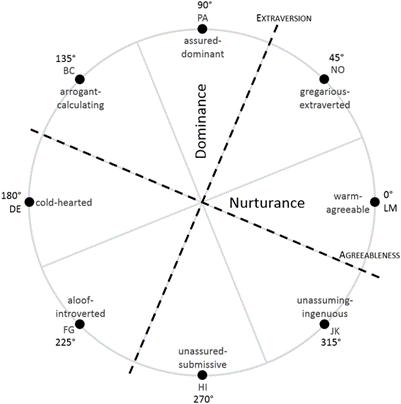
\includegraphics[width=12cm]{img/circumplex_wiggins.png}
    \caption{Le Circomplexe interpersonnel de Wiggins (1995) et le Modèle à 5 facteurs ou \textit{Big Five}}
    \label{circumplex_wiggins}
\end{figure}
\newpage


Comme apparent sur le cercle, les axes de l'agréabilité et de l'extraversion du \textit{Big Five} sont en effet situés à environ 45 degrés des axes familiers de l'amour et du statut de ce circomplexe, et semblent donc traiter d'aspects différents des mêmes dimensions latentes. A titre de remarque, l'extraversion est définie dans le modèle des \textit{Big Five} comme une activité tournée vers l'extérieur, mais non comme un « comportement prosocial » (elle ne décrit pas, par exemple, à quel point une personne se soucie sincèrement des autres). C'est l'agréabilité qui fait précisément office de liant social, caractérisant quant à elle des personnes plus tolérantes, douces, indulgentes, agréables, altruistes et obligeantes. 

L'agréabilité et l'extraversion se rapporteraient ainsi plus étroitement au comportement interpersonnel que les mesures des domaines restants du NEO-PI (névrosisme, conscienciosité et ouverture à l'expérience). Pour autant, nous avons également inclus dans les traits de personnalité préférentiellement associés à l’agentivité qui nous intéressent ici la conscienciosité, sur la base d’un certain nombre de travaux plus récents\footnote{\cite{hurley_agency_1998}\footnote{\cite{abele_facets_2016} - en notant que dans cette étude et en dépit de la définition retenue dans le \textit{Big Five}, l'extraversion est également associée à la Communion. Cela rend donc l'ajout la consciensioté plus pertinent encore, afin que notre méthode de validation externe ait toutes les chances d'être concluante}}. De la même façon, outre l'agréabilité, l'ouverture y est parfois positivement corrélée avec la communion, et est donc également prise en compte dans notre étude.

\section{Outils utilisés}

Bien que nous détaillions de manière exhaustive les composantes de l’indice global d’agentivité dans le chapitre suivant, elles sont récapitulées et réparties ici dans des catégories définies sur la base des différentes facettes du concept d’agentivité mentionnées plus tôt, et qui ont pour partie inspiré la sélection de ces différents éléments linguistiques supposés avoir trait à l’agentivité :  

\begin{center}
\begin{table}[ht]
\caption{Récapitulatif des marqueurs linguistiques retenus}
\bigskip
\renewcommand{\arraystretch}{1.5} % Adjust the value as needed
\begin{tabular}{ |p{3cm}|p{3cm}|p{3cm}|p{3cm}|p{3cm}|p{3cm}| }
 \hline
 \textbf{Sentiment d'agentivité} \newline{Locus de Contrôle} &  \textbf{Efficacité de l'action*} \newline{Disposition objective à l'action} & \textbf{Volition} \newline{Degré de connotation agentive des évènements décrits} & \textbf{Identification à l'action} \newline{Degré de référence à soi} & \textbf{Compréhension globale} \newline{Capacité de distanciation psychologique}  \\
 \hline
 \textit{Verbes} &  Agentivité grammaticale (orateur-sujet) & Transitivité & Pronoms (individuels vs. collectifs, à la 1ère personne) & Modes irréels \\
    Voix active vs. passive & \textit{Verbes} & Télicité & Déictiques (proximaux vs. distaux) & Alternance de temps \\
    Modalité (interne vs. externe) & Evènements vs. états & Adverbes intentionnels & & Degré d'abstraction (adverbes, mots-outils, adjectifs)\\
 \hline
\end{tabular}
\end{table}
    \label{recap_marqueurs_agentifs}
\end{center}
\vspace{-20pt} % Adjust the value to reduce the space
\textit{* L’agentivité telle que nous la comprenons, et contrairement à Hopper et Thompson\footnote{\cite{hopper_transitivity_1980}}, ne semble pas impliquer l'accomplissement le plus total de l'action, et/ou l'affectation la plus complète de l'objet s'il y en a un, mais plutôt la possibilité (le « pouvoir » de l'agent) et l'actualité d'une telle action (le fait qu'il y ait une action évoquée, plutôt qu'un état), ces deux concepts définissant l'efficacité de l'action, à laquelle l’agentivité ne saurait par ailleurs se réduire.}


Dans le tableau ci-dessus, la direction prédite est toujours positive, à savoir que chaque indicateur est supposé être positivement corrélé avec le niveau d’agentivité du personnage locuteur. En italique sont mentionnés les indicateurs pour lesquels la direction est ambigüe. La mention « vs.» signifie que la métrique consiste en un ratio entre les deux notions mises en rapport (calculé dans l'ordre d'apparition de ces dernières). Par exemple, la métrique « Voix active vs. passive » est égale au ratio (nombre d'occurrences de la voix active)/(nombre d'occurrences de la voix passive). Enfin, lorsque cette mention « vs. » apparait entre parenthèses, cela signifie qu'une métrique existe également pour compter le nombre total d'occurrences du marqueur en question (en plus du ratio mentionné). A titre d'exemple, notre indice agentif inclut à la fois une métrique calculant la fréquence totale des déictiques dans les répliques étudiées, et une métrique calculant le ratio (nombre de déictiques proximaux)/(nombre de déictiques distaux) dans ces dernières.

Concernant l’analyse textuelle, nous avons utilisé le modèle \textit{fr-dep-news-trf} de spaCy\footnote{\url{https://spacy.io/}}, ainsi que le modèle \textit{fr} de pie-extended\footnote{\url{https://github.com/hipster-philology/nlp-pie-taggers}}. Chacun des marqueurs linguistiques a été normalisé en fonction du nombre total de mots prononcés respectivement par les personnages haut et bas statut, dans chaque pièce, à l'exception : 

-des signes de ponctuation individuels (rapportés à la ponctuation totale) ; 

-des verbes conjugués (cette métrique, ainsi que celle mesurant le gérondif spécifiquement), modaux, transitifs, « statifs » et copules, des verbes dont le sujet est à la première personne et des marqueurs de négation (rapportés au nombre total de verbes) ; 

-des métriques de temps et modes (subjonctif etc) (rapportées au nombre total de verbes conjugués)

-du marqueur d’agentivité grammaticale (rapportée au nombre total de phrases) ;

-des duplicata d’indicateurs pour lesquels la contrainte d’avoir un sujet à la première personne nous semblait pertinente à ajouter (rapportés au nombre total de verbes ayant un sujet à la première personne) 

-et des ratios, a fortiori.

\part{Détail des composants linguistiques retenus}

\chapter{Actionnalité, volition et locus de contrôle : une escapade sémantique}

Nous adoptons ici une approche en priorité « structurelle »  du langage, plutôt que sémantique, c'est-à-dire que nous nous limitons aux niveaux grammatical et syntaxique pour la majeure partie de notre analyse. L'idée est de se concentrer de préférence sur ce qui, dans la langue, manifeste l'état d'esprit qui la sous-tend, et qui guiderait supposément l'utilisation de ses composants les plus structurels indépendamment du contenu sémantique particulier exprimé par le locuteur.

Néanmoins, il semble qu'il faille mentionner quelques travaux antérieurs de nature sémantique, en ce qu'ils sont étroitement liés à notre question de recherche, et bien qu’ils présentent des limites qui justifieront, selon nous, une focalisation ultérieure sur les éléments les plus structurels du discours.

\section{Les limites d’une analyse par mot-clé}

Sur la base des travaux de Pietraszkiewicz\footnote{\cite{pietraszkiewicz_big_2019}}, une analyse lexico-sémantique exploratoire aurait pu consister à simplement compter, pour chaque groupe de répliques de personnages « haut »  et « bas » statut, la fréquence relative de tous les lemmes inclus dans son dictionnaire d’agentivité, comme a pu le faire Seligman dans son étude de la Bible\footnote{Seligman, M., Maymin, P., « Agency in the Bible » (2022)}.

\begin{table}[H]
\caption{Dictionnaire de l’Agentivité de Pietraszkiewicz}
\centering
\bigskip
\begin{tabular}{|p{0.8\linewidth}|}
    \hline
    Mots \\
    \hline
    able accomplish* accurac* accurate* achiev* acquir* actualiz* adaptab* adept* ambition* ambitious* aptitude* aptly aptness aspiration* aspire* aspiring assert* attain* authoritative* autonomous* autonomy capab* careful* choice choices clever* compet* completion confident confidently conquer* conscientious* contemplat* contend* contest* decid* decision* decisive* defeat* deliberat* dependable determin* difficult* do doable doing eager* earn earned earning earns easiness easy effective* efficien* effort* empowered enact* endeavor* establish established establishes establishing exact* expert* fail* fluen* freedom* freely goal goal-oriented goals importan* independ* individualist insight* intent* intuition intuitive* keen* know* liberties liberty logic* loner* made make makes making mastered masterful* mastering mastery motivat* need needed needing needs objectiv* obtain* opportun* overcame overcome overcomes overcoming persever* persist* persistent pioneer* practic* pragmat* prevail* pride prideful* priorit* proactive* productive* productivity proficien* prosper* proud* purpose* pursu* rational* realiz* rebel* recog* reliab* reputation* resilien* resolute* resolution resolv* responsib* reward* risk* savv* score scored scores scoring self self-* should* significant* skill skilled skillful* skills* smart smartly steadfast* strive* striving* struggl* stubborn* succeed* success* sure take takes taking tenac* think thinking thinks thought took tried tries triumph* trying unaided unyielding* vanquish* victor* will willing* willpower win winner* winning* wins wit wits witting* won won't you you'* your yours yourself \\
    \hline
\end{tabular}
 \label{Tab:dico_pietra}
\end{table}

\begin{table}[ht]
\centering
\bigskip
\renewcommand{\arraystretch}{1.5} % Adjust the value as needed
\begin{tabular}{|c|p{10cm}|}
    \hline
    Catégorie & Mots \\
    \hline
    Agentivité & tried, victory, knowing, wit, pride, obtain, willing, choice, thinking, purposes, freedom, resolved, needs, opportunity, easy, determined, doing, success, obtained, established, sure, taking, liberty, need, knowledge, making, purpose, able, self, took, known, think, thought, know, take, make, your, do, should, made \\
    \hline
    Efficacité & able, many, some, which, have, having, but, also, these, those \\
    Optimisme & things, good, joy, yet, hope (mais pas “no hope”) \\
    Imagination & desire, new, truth, true, false, ask, asked, know, known \\
    \hline
\end{tabular}
\caption{Les mots agentifs retenus par Seligman}
 \label{Tab:dico_seligman}
\end{table}
\newpage

\bigskip

Cette liste aurait d'ailleurs pu être complétée par les travaux de Rouhizadeh\footnote{\cite{rouhizadeh_identifying_2018}}, ce dernier ayant démontré qu'un locus de contrôle interne était associé à des verbes indiquant une « tentative » (\textit{attempt} en anglais), tandis qu'un locus de contrôle externe serait associé à des verbes de cognition, de manque, de sentiments et d'espoir : 

\begin{figure}[H]
\centering
    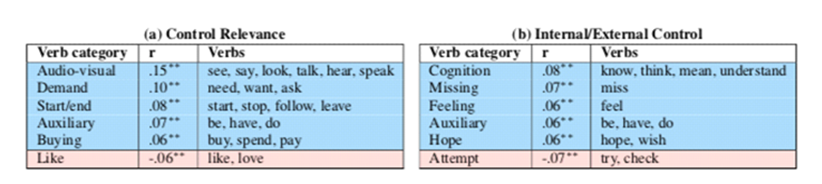
\includegraphics[width=16cm]{img/verbs_locus.png}
    \setlength{\abovecaptionskip}{-2pt} % Adjust the length to your preference
    \caption{Rouhizadeh et al. (2018) - Coefficients de régression logistique entre les catégories de verbes et le contrôle (les valeurs positives correspondent à la pertinence du contrôle et au contrôle externe). ** : p< 0,01 après correction de Benjamini-Hochberg. Les caractéristiques ayant des coefficients positifs sont en bleu et celles ayant des coefficients négatifs sont en rouge}
    \label{verbs_locus}
\end{figure}

Néanmoins, et outre le fait que ces études ont été menées en anglais et non en français, la principale limite d’une analyse sémantique réside dans sa vulnérabilité aux variations historiques de sens.

Certes, une analyse sémantique latente (LSA) aurait pu servir à calculer la similarité sémantique entre chaque mot unique d'un texte ou d'un énoncé, et un nombre limité de \textit{seed-words}\footnote{\cite{diuk_quantitative_2012}}, ce pour chaque groupe de répliques dans une pièce considérée. Il aurait également été possible de s’inspirer de la méthode « historiquement verrouillée »  de Snefjella\footnote{\cite{snefjella_historical_2019}}, afin de s'assurer de la stabilité sémantique, dans le temps, des \textit{seed-words} retenus.

Pour autant, ce travail dépassait largement le cadre de notre projet de recherche actuel, qu’il aurait fait reposer sur des méthodes d’analyse elles-mêmes exploratoires dans le cas de Snefjella. Aussi, notre paradigme et l’approche inspirée d’Hopper et Thompson\footnote{\cite{hopper_transitivity_1980}} justifiaient de se concentrer principalement sur les marqueurs linguistiques infra-sémantiques. 

\section{Les adverbes intentionnels, statut hybride ?}

La volition étant un aspect important de l'agentivité qu’il serait difficile d’analyser autrement que par une approche sémantique, nous avons cependant décidé de définir et de mesurer l'occurrence relative d'une liste d'adverbes univoquement intentionnels. Ceux-ci présentaient l'avantage d'être en nombre relativement limité dans la langue française, et d'avoir un sens \textit{a priori }historiquement stable.

\begin{table}[ht]
\caption{Expressions adverbiales à valeur intentionnelle retenues}
\centering
\bigskip
\renewcommand{\arraystretch}{1.5} % Adjust the value as needed
\begin{tabular}{|p{0.8\linewidth}|}
    \hline
     « volontairement », « délibérément », « expressément », « intentionnellement », « sciemment », « à dessein », « exprès »   \\
    \hline
\end{tabular}
 \label{Tab:adv_intention}
\end{table}

\section{La modalité : entre sémantique et pragmatique}

En guise de clôture de cette escapade sémantique, nous avons également examiné les marqueurs modaux utilisés dans les répliques de chaque groupe de personnages. 

La modalité est un concept linguistique qui s'intéresse au statut de la proposition décrivant l'événement\footnote{\cite{palmer_mood_1986}}, ou plutôt à l'attitude qu'un locuteur peut avoir vis-à-vis d'un événement ou d'un état. Une phrase modalisée situe une proposition sous-jacente, ou préjacente, dans l'espace des possibilités, décrivant des événements avec des informations supplémentaires telles que leur degré de désirabilité, de plausibilité ou de faisabilité.

Dans son sens le plus restrictif, la modalité est ainsi une « catégorie de signification linguistique ayant à voir [spécifiquement] avec l'expression de la possibilité et de la nécessité »\footnote{\cite{von_fintel_modality_2006}}.

On distingue traditionnellement deux grands types de modalité, qui nous intéressent particulièrement ici : la modalité épistémique (également appelée subjective ou hypothétique) et la modalité non épistémique, parfois appelée « orientée vers l'agent » (\textit{agent-oriented}), ou encore « racine déontique »  (\textit{deontic root}), « objective »  ou « pragmatique ».

La modalité épistémique concerne ce qui est possible, plausible ou nécessaire compte tenu de ce qui est connu et des preuves disponibles. Grâce à cette modalité, les locuteurs expriment un jugement sur le statut factuel de la proposition.

La modalité non épistémique est pour sa part composée de deux sous-modalités principales : l'une se concentrant sur les capacités objectives et le déroulement dynamique des événements (Palmer, 1986), parfois appelée  « modalité circonstancielle » ; et l'autre ayant avoir avec les raisons subjectives de donner la priorité à un événement plutôt qu'à un autre\footnote{\cite{portner_modality_2010}}, pour laquelle il existe d'autres subdivisions selon que l'événement est priorisé en termes de normes (« déontique »), de désirs/préférences (« boulétique »), ou de buts (« téléologique »).

A noter que Bybee et al.\footnote{\cite{bybee_evolution_1995}} ont élaboré leur propre classification s'agissant de la modalité « orientée vers l'agent », identifiant quatre sous-types : (i) l'obligation, (ii) la nécessité, (iii) la capacité et (iv) le désir. Ces auteurs discutent également d'un certain nombre de ressources pour représenter les connaissances des locuteurs ainsi que leur position à l'égard des événements et des états de fait. En particulier, l'utilisation de verbes modaux tels que les verbes anglais \textit{must}, \textit{should}, ou \textit{may} permettrait aux auditeurs de comprendre comment les locuteurs représentent leurs propres obligations ainsi que celles des autres dans un monde moral principalement construit par la langue (ou plutôt le discours). L'utilisation de prédicats de volition tels que \textit{want}, \textit{would}, \textit{would like}, ou \textit{wish}, pour leur part, mettrait certains états psychologiques internes à la disposition des autres pour qu'ils les comprennent et les évaluent. 

Ainsi, quelle que soit la taxonomie, la « modalité orientée vers l'agent » rend compte, par l'utilisation de verbes modaux en particulier, de l'existence de conditions internes et externes à l'accomplissement de l'action exprimée dans le prédicat principal. Avec cette définition, la modalité semble donc particulièrement liée à notre notion d’agentivité.

Cela étant, la modalité ultimement projetée par le locuteur, et/ou comprise par l'auditeur, dépend en réalité du contexte de l'occurrence, les verbes modaux seuls se révélant intrinsèquement polysémiques, ou du moins ambigus. A titre d’exemple, \textit{devoir} dans « Il devrait pleuvoir demain » a une connotation épistémique, tandis que « les visiteurs doivent partir à 6 heures »  est plutôt déontique, « Tu te dois d’y aller »  boulétique, « Pardon, je dois éternuer »  circonstancielle, et « Pour rentrer à temps, tu devrais prendre un taxi »  téléologique.

Pour déterminer la modalité d’une clause dans une perspective compositionnelle, Warsnby\footnote{\cite{warnsby_coding_2006}} détaille ainsi les caractéristiques, au-delà des verbes modaux et dans cet ordre de désambiguïsation, qui constitueraient ce qu'elle appelle la « contrôlabilité » du participant, définie comme « la capacité d'un agent à choisir de provoquer la situation référentielle représentée par les propositions des phrases »\footnote{\cite{klinge_impact_1996}}, et qui correspond étroitement à notre définition de l’agentivité, entendue dans un sens linguistique plus étroit. On précisera à nouveau que ces composantes ont été établies pour l'anglais seul. Cela dit, et compte tenu de l’inexistence de telles analyses appliquées au français, il semblait raisonnable d’y puiser une source d’inspiration, à supposer que leurs équivalents français soient interprétés de la même façon par des lecteurs francophones, ce à quoi ce mémoire tente précisément de répondre, \textit{in fine}.

Premièrement, la présence d'un adverbe de but (souvent une clause, comme dans « afin de [faire quelque chose] ») indiquerait une lecture non épistémique. Inversement, les adverbes modaux épistémiques tels que \textit{possiblement}, \textit{peut-être}, \textit{sûrement}, etc., peuvent qaunt à eux neutraliser, désambiguïser ou renforcer l'interprétation épistémique du modal dans un énoncé. Comme mentionné dans la section précédente, nous avons donc créé une mesure distincte pour les adverbes intentionnels, ainsi que pour les adverbes de doute et d'affirmation (chaque fois identifiés par l'usage d'expressions régulières).

\vspace{-40pt}

\begin{table}[H]
\caption{Expressions adverbiales à valeur de doute retenues}
\centering
\bigskip
\renewcommand{\arraystretch}{1.5} % Adjust the value as needed
\begin{tabular}{|p{0.8\linewidth}|}
    \hline
    « apparemment », « peut-être », « peut être », « probablement », 
    « vraisemblablement », 
    « éventuellement »,
    « supposément »,
    « présumément »,
    « possiblement »,
    « potentiellement »,
    « hypothétiquement »,
    « a priori », 
    « sans doute », 
    « si jamais »,
    « toutefois », 
    « certainement »   \\
    \hline
\end{tabular}
 \label{Tab:adv_doute}
\end{table}

\begin{table}[H]
\caption{Expressions adverbiales à valeur d'affirmation retenues}
\centering
\bigskip
\renewcommand{\arraystretch}{1.5} % Adjust the value as needed
\begin{tabular}{|p{0.8\linewidth}|}
    \hline
    « à vrai dire », « assurément », 
    « à coup sûr »,
    « absolument »,
    « bien sûr »,
    « pour sûr »,
    « sans conteste »,
    « sans contredit »,
    « bien entendu »,
    « effectivement », 
    « en effet »,
    « exactement »,
    « parfaitement »,
    « clairement »,
    « certainement »,
    « évidemment »,
    « fatalement »,
    « forcément »,
    « immanquablement »,
    « indubitablement »,
    « inéluctablement »,
    « inévitablement »,
    « infailliblement »,
    « sûrement »,
    « certes », 
    « en vérité », 
    « oui »,
    « précisément », 
    « sans doute », 
    « nul doute »,
    « sans aucun doute »,
    « sans le moindre doute »,
    « si fait », 
    « tout à fait »,
    « si. », « Si, », « Si : », « Si ! », 
    « soit. », « soit, », « soit : », « soit ! »,
    « volontiers », 
    « vraiment », 
    « naturellement », 
    « vraisemblablement »,
    « d'accord »   \\
    \hline
\end{tabular}
 \label{Tab:adv_affirmation}
\end{table}
\bigskip

En outre, la contrôlabilité sélectionnerait un agent non générique plutôt que générique, à savoir un agent animé, qui peut être approximé par les pronoms personnels (notamment au théâtre), ou un agent défini, approximé par le nombre de déterminants définis (bien que ce proxy soit très imparfait). Elle sélectionnerait également les événements (y compris les changements d'état), principalement interprétés comme déontiques, plutôt que les états (le plus souvent épistémiques), ce qui est encore une fois en alignement avec certaines de nos considérations théoriques au moment de sélectionner les marqueurs linguistiques de l’agentivité, notamment l’inclusion d’un ratio des verbes statifs par rapport aux autres verbes  (voir la partie \textit{III. 2.3. Analyse des dépendances syntaxiques}). A cela, nous ajoutons ainsi pour le calcul de l’indice agentif une métrique comptant le nombre relatif de pronoms personnels, ainsi qu’une métrique rapportant le nombre de déterminants définis à ceux indéfinis, sur la base des propositions de Warsnby.

Selon l’auteur, il s'agirait là des conditions explicites rendant inefficace l'influence d'autres caractéristiques.

Lorsqu’elles sont absentes, il est encore possible d’examiner les verbes modaux utilisés spécifiquement comme verbe matrice (c.a.d. principal) d'une clause de complément finie, qui reçoivent généralement une lecture épistémique. 

En outre, l'on peut supposer que les énoncés déontiques ont généralement une transitivité plus élevée que les énoncés épistémiques. Ceci est, une fois de plus, cohérent avec nos propres mesures (voir la partie \textit{III. 2.3. Analyse des dépendances syntaxiques}).

« Les situations situées dans le temps passé et les situations situées au moment de l'énonciation (progressives) seraient immuables, et donc hors du contrôle de l'agent », et interprétées comme épistémiques\footnote{\cite{klinge_impact_1996}}. Inversement, lorsque le temps de référence est postérieur au temps de la modalité exprimée, l'interprétation déontique serait possible (mais pas nécessaire). Il semblait toutefois trop complexe d’implémenter ce critère de façon efficiente, même en l’approximant.

En ce qui concerne la modification aspectuelle, la télicité sélectionnerait de préférence une interprétation déontique, et l'atélicité une interprétation épistémique. En particulier, le passé simple décrirait les événements en fonction du contexte (déontique), tandis que le passé composé ne donnerait qu'une information stative (épistémique). Comme cela est suggéré dans une autre partie de notre analyse (voir la section \textit{III. 2.2. Pronoms et déictiques : la référence au soi} notamment), nous avons inclus des métriques s'intéressant aux temps verbaux utilisés.

Enfin, la présence de la voix passive favoriserait une interprétation épistémique en indiquant un manque de contrôle de la part du sujet, mais aussi la stativité de la situation décrite, ce qui est encore une fois cohérent avec le lien entre  voix active et agentivité supposé plus bas (voir la partie \textit{III. 2.3. Analyse des dépendances syntaxiques}). 

 Warsnby note finalement que les énoncés contenant \textit{must}, (\textit{maste}), \textit{may} ou \textit{can} en anglais, dans lesquels les propositions sont codées de manière à indiquer un manque de contrôle de la part de l'agent, sont bien interprétés de manière épistémique. Dans les énoncés où les caractéristiques pertinentes indiquent que l'agent visé contrôle la situation dénotée par la proposition, en revanche, l'interprétation préférée est déontique.

Cela étant, nous n'avons en réalité pas pu analyser la modalité de manière compositionnelle comme nous le faisons pour la télicité (\textit{III. 3.1. L’analyse aspectuelle de la télicité}), en la définissant pour chaque clause spécifique, ce en raison d' un manque de temps et d'une trop grande complexification technique. Nous avons donc choisi d'estimer plutôt la modalité apparaissant comme la plus récurrente, au niveau global, dans chaque groupe de répliques, en se focalisant sur les verbes modaux, potentiellement modulés par les quelques proxys retenus plus haut. Ceci rend notre approche de la modalité particulièrement limitée, l’interprétation des verbes modaux étant dans une large mesure déterminée par l'ensemble de la construction dans laquelle ils s’inscrivent, à l’échelle de chaque clause. 

Il reste que l'on peut supposer de façon raisonnable que ces verbes modaux ont une signification préférentielle. En effet, une gradation intuitive semble exister entre les modaux signifiant une obligation (\textit{devoir}, \textit{avoir besoin de}, \textit{être supposé faire} etc. - tous ces éléments atténuant l'agentivité et se référant à un locus de contrôle externe), une possibilité (\textit{pouvoir}, notamment au conditionnel, \textit{être susceptible} de etc.), une capacité (\textit{être capable de}, \textit{pouvoir} à l'indicatif), un désir (\textit{vouloir} [que quelqu'un fasse quelque chose], \textit{désirer}, \textit{aimer}, \textit{souhaiter} au conditionnel notamment etc.) ou une action à venir (\textit{être sur le point de},\textit{ être en train de}, l'emploi du futur etc. - les marqueurs de futurité se chevauchent avec la modalité car ils impliquent une certaine forme d'incertitude). En outre, les modaux utilisés en référence à l'agent et aux règles ou normes (déontiques), qui nous intéressent particulièrement, semblent précisément revêtir les sens les moins ambigus\footnote{\cite{nesselhauf_mechanisms_2012}}.

Pour autant, et compte tenu de notre seconde question de recherche diachronique, il est nécessaire de s'assurer que ces corrélations sémantiques préférentielles sont à peu près stables dans le temps.

Dans plusieurs de ses études, Hilpert\footnote{\cite{hilpert_change_2016}; \cite{hilpert_disentangling_2021}} utilise la modélisation de l'espace vectoriel sémantique fondée sur les tokens pour déterminer si différents auxiliaires modaux peuvent être distingués en termes de profils dits « collocationnels » (ce que l'on appelle la « sémantique distributionnelle »), et si différents sens du même auxiliaire présentent des préférences collocationnelles divergentes.  

Il constate, pour l'anglais, que les paires quasi-synonymes d'expressions modales, telles que \textit{may} et \textit{might}, ou \textit{must} et \textit{have to}, diffèrent dans leurs caractéristiques distributionnelles. En outre, \textit{may} en particulier aurait subi un changement sémantique continu, s'éloignant des significations modales déontiques et des utilisations textuelles « impliquées » (\textit{involved} en anglais) pour se rapprocher des significations épistémiques et d'un degré plus élevé d'informativité. En bref, les collocats verbaux les plus fortement attirés par \textit{may} au XIX\ieme ~siècle se prêtent à l'expression d'un sens permissif, tandis que les collocats les plus fréquents dans les données plus récentes se combinent avec \textit{may} pour exprimer des possibilités. 

Plus généralement, les aires sémantiques qui contiennent des verbes aux significations abstraites et épistémiques seraient en augmentation. Cela étant, \textit{must}, par exemple, est encore utilisé relativement plus souvent avec un sens déontique. Aussi, Hilpert conclut qu'en tant qu'éléments hautement grammaticalisés, les auxiliaires modaux anglais présentent une assez grande variabilité collocationnelle, mais que sous la surface de cette variabilité, il existe une multitude d'associations qui lient conventionnellement une expression modale donnée à un ensemble particulier d'éléments lexicaux, ou un sens modal spécifique à un contexte linguistique particulier. Ainsi, bien qu'il existe des changements sémantiques, Hilpert peut affirmer que \textit{might}, \textit{must} et \textit{could} ont globalement plus de potentiel épistémique, tandis que \textit{can} et \textit{will} sont stables en termes de sens et déontiques. Pour sa part, \textit{would} demeure assez ambivalent. Alors que \textit{will} n'a pas d'équivalent direct en français, l'analyse du modal \textit{pouvoir} (équivalent de \textit{can}) semblait donc particulièrement pertinente pour notre question, en considérant qu’il possède, en français également, un sens déontique relativement stable.

Mais pour complexifier encore l'analyse, la corrélation de ces verbes modaux avec le degré d’agentivité personnelle, sur la base de la gradation mentionnée plus haut, n'est en réalité pas évidente. La tragédie grecque illustre bien cette inéquation. Bien qu'il s'agisse d'un cas limite du point de vue du locus de contrôle des personnages, apparemment manifestement externe puisque ces derniers sont soumis à la contingence divine (bien que l'on trouve déjà, dans certaines tragédies, des expressions ambiguës telles que le « désir de sacrifice » d'Agamemnon\footnote{\cite{vernant_j-p__vidal-naquet_p_mythe_2005}}), d’aucuns pourrait considérer que ces mêmes personnages identifient en réalité les vexations divines à leur propre destin (faisant tout le tragique de la pièce, précisément). De fait, ils construisent souvent des récits \textit{a posteriori} pour donner un sens à leurs souffrances, et expriment en ce sens une capacité à interpréter cette contingence dans des termes personnels, caractéristique d’un haut niveau d’agentivité.

De la même façon, comme le suppose Rymes\footnote{\cite{rymes_construction_1995}} dans une étude socio-linguistique s'attachant à analyser le discours de jeunes adolescents ayant abandonné l'école secondaire dans les années 90, pour continuer à se considérer comme de bonnes personnes malgré les actes criminels qu'ils ont commis, ces mêmes jeunes atténuent paradoxalement l'agentivité réelle induite par leur langage, principalement par l'utilisation de verbes modaux associés à un locus de contrôle externe, dans un acte qui pourrait pour sa part être considéré comme particulièrement agentif (ce que Rymes appelle « l'agentivité morale »).

C'est en ce sens que nous avons décliné notre métrique s’attachant aux verbes modaux de différentes manières. En trouvant les équivalents français les plus directs par recoupement de grammaires françaises bien connues et accessibles en ligne\footnote{\cite{jacqueline_ollivier_martin_beaudoin_grammaire_2007}; \cite{cedrick_fairon_maurice_grevisse_petit_2018}; \cite{delatour_nouvelle_1991}}, nous avons tout d'abord inclus une métrique comptant le nombre relatif de verbes modaux globalement utilisés, comme approximation de l’agentivité discursive ou morale des personnages considérés, ce quel que soit le contrôle sur l’action sémantiquement impliqué par le verbe modal en question. Nous avons en réalité calculé deux versions différentes de cet indicateur, l'une restrictive se concentrant sur les modaux d'obligation/permission et de désir (« pouvoir », « devoir », « vouloir », « falloir} + infinitif) et l'autre plus large (contenant également « espérer », « savoir », « penser », « aller » + infinitif). 

Nous avons également, au moyen d’une nouvelle métrique, opposé l'utilisation personnelle des modaux (à savoir ceux dont le sujet est à la première personne) à leur utilisation globale. En effet, cette utilisation « structurelle » des modaux, qui ne tient pas compte de leur contenu sémantique, pourrait n’être pertinente que lorsqu'on parle de soi (l’agentivité discursive ou morale se restreignant potentiellement aux seuls récits identitaires).

A cela, nous avons enfin ajouté une métrique calculant le rapport entre les modaux traduisant un locus de contrôle interne (« pouvoir », « vouloir » + infinitif), et externe respectivement (« devoir », « falloir » + infinitif), étant donné leur connotation agentive plutôt univoque et stable dans le temps, en tenant compte cette fois du contrôle sémantiquement impliqué par le modal employé. 

L’idée d’une utilisation des verbes modaux d'abord « performative », et en cela partiellement indépendante de leur contenu sémantique, est d'ailleurs corroborée par l'observation de tendances globales dans l'utilisation des verbes modaux, ayant affecté chacun d'entre eux de façon indistincte. De nombreux articles\footnote{\cite{myhill_change_1995}}\footnote{\cite{smith_changes_2003}}\footnote{\cite{leech_change_nodate}}\footnote{\cite{aarts_modals_2013}} ont en effet constaté un déclin général de la fréquence d'utilisation des verbes modaux au cours du XX\ieme ~siècle au moins, bien que ce phénomène pourrait être compensé par une augmentation globale parallèle de l'utilisation des verbes semi-modaux en anglais (à l'exception de \textit{have got to}). En particulier, ces travaux observent que \textit{will} et \textit{must} sont les verbes qui diminuent le plus drastiquement, tandis que l’utilisation de \textit{need} et \textit{be going to} (semi-modaux) augmente. Il s’agirait donc plutôt d'un glissement que d'une disparition pure et simple de la modalité. Pour autant, ce dernier souligne la limite de notre métrique comptant simplement le nombre total de verbes modaux utilisés, qui ne saurait se suffire à elle-même à l'heure où l'expression de la modalité se ferait plus discrète.

Plus problématique encore pour notre analyse, et comme le suggèrait Hilpert, il semblerait que l’on assiste au déclin du sens « intentionnel » (en anglais \textit{'speaker’s intention’-sense}) des modaux, notamment pour \textit{will}, ce en faveur d'un sens de « pure prédiction » (\textit{'pure-prediction’ sense}\footnote{\cite{nesselhauf_mechanisms_2012}}, sur la base de ses seules interprétations cependant, et d’un échantillon restreint d’expressions analysées), ce qui est cohérent avec le Bybee-path, aussi appelé processus de « grammaticalisation », une tendance inhérente à la langue dans son ensemble. Selon Bybee\footnote{\cite{bybee_evolution_1995}}, en cherchant à exprimer un sens plus spécifique, une langue finirait paradoxalement par « blanchir » (\textit{bleaching} en anglais), autorisant alors une plus grande acceptabilité contextuelle avec le temps, de sorte que de nombreuses significations se retrouvent à co-occuper dans un seul mot. Ainsi, plus une expression temporelle future est ancienne par exemple, plus elle exprimerait fréquemment une prédiction non colorée par la caractéristique de l'intention. Le déclin de l'expression de l'intention du sujet et du locuteur avec les marqueurs de futur résulterait donc de changements successifs entre les expressions de temps futur établies, et les nouvelles constructions venant prendre le relais pour exprimer les significations en question à mesure que les expressions de temps futur plus anciennes, du moins celles qui proviennent du matériel lexical, évoluent sur le chemin de Bybee pour exprimer la « prédiction pure ». 

Aussi, comme le note Nesselhauf\footnote{\cite{nesselhauf_mechanisms_2012}}, les deux types de changements sont probablement motivés, au moins en partie, par des transformations socioculturelles et stylistiques. En particulier, une explication souvent avancée pour rendre compte de ce moindre usage des verbes modaux, ou du moins de leur moindre explicitation des intérêts du locuteur, est celle de la « démocratisation de l'anglais » (les études ne s'intéressent là encore qu'à l’anglais seul). Cette dernière fait référence à une « montée d'alternatives plus conviviales et moins menaçantes, dans une société apparemment plus égalitaire, démocratique et antiautoritaire » qui conduirait à une « tendance des locuteurs à éviter les modes d'interaction inégaux », notamment les marqueurs manifestes d'autorité dans les énoncés véhiculant une directive (Farrelly et al., 2012). Cela expliquerait la préférence pour les modaux exprimant une obligation médiane, comme \textit{need to,} afin d'éviter les marqueurs de pouvoir excessifs tels que \textit{must}. Une construction de la forme \textit{X needs you to} serait ainsi interprétée comme un appel plutôt que comme un ordre direct, psychologisant par-là les directives (certains parlent de « pseudo-démocratisation »).

D’autres phénomènes pourraient encore soutenir, selon Nesselhauf, le déclin du sens intentionnel de \textit{will} en particulier. Tout d'abord, une expression qui n’est pas traditionnellement une expression de futurité mais avec un sens intentionnel similaire pourrait avoir remplacé l'utilisation d'expressions du futur avec ce sens dans certains contextes. En effet, il semble qu'en anglais, \textit{be going to} et le \textit{present progressive} aient remplacé \textit{will} et \textit{shall}, dans une certaine mesure, pour exprimer une prédiction fondée sur l'intention du sujet. En ce sens, nous avons inclus une métrique mesurant l'utilisation du progressif, correspondant en français à l’expression « être en train de [faire quelque chose] ». En outre, la construction \textit{want to} est identifiée par Nesselhauf comme un marqueur de futurité émergent, qui a commencé à être utilisé pour des prédictions fondées sur l'intention du sujet.

Autre possibilité avancée par l'auteur, ce déclin pourrait en partie s’expliquer par un changement stylistique global: alors que dans les exemples du XVIII\ieme ~siècle, le sujet des clauses intentionnelles (avec \textit{shall}) diffère du locuteur, de sorte que seule l'intention du locuteur et non celle du sujet est exprimée, en anglais actuel, il semble beaucoup plus probable que l'on choisisse une construction où le locuteur et le sujet sont totalement ou partiellement identiques (c'est-à-dire avec \textit{I} ou \textit{we}, en anglais, comme sujet – l’auteur compare par exemple \textit{My friendship to you shall be steady} avec \textit{I'm always going to be your friend}). Et cela refléterait une tendance plus générale à passer de modes d'expression impersonnels à des modes d'expression plus personnels dans de nombreux types de textes. La diminution globale de la construction passive va également dans ce sens\footnote{\cite{leech_change_nodate}} ; et il est intéressant de constater que c'est principalement au théâtre et dans la conversation fictionnelle que le déclin a eu lieu\footnote{toutes ces observations s'appuient sur le Corpus ARCHER : \url{https://www.projects.alc.manchester.ac.uk/archer/}}.

Enfin, comme l'indique Nesselhauf, « les personnages de fiction pourraient être de plus en plus représentés comme se sentant davantage déterminés par les circonstances extérieures et comme ayant le sentiment que leurs intentions personnelles et celles des autres ont moins d'influence sur ce que l'avenir pourrait leur apporter. Et cela pourrait refléter une évolution plus générale, qui ne se limite pas à la représentation littéraire : à mesure que le réseau d'interconnexions dans la société devient de plus en plus complexe et dense (cf., par exemple, Elias 2000), l'intention propre d'un sujet pourrait avoir moins d'influence sur les événements futurs ou du moins pourrait amener les sujets à supposer que c'est le cas ». Cette affirmation est particulièrement contradictoire avec nos propres hypothèses. Néanmoins, il faut d'abord noter que dans l'analyse de Nesselhauf, ce sentiment potentiel de moindre contrôle sur les événements futurs ne s'étend en réalité pas aux prédictions fondées sur des arrangements pour lesquels le sujet a été personnellement impliqué, ce qui semble difficilement explicable selon la lecture précédente.

A partir de là, et en maintenant la validité de notre analyse modale, nous proposons une interprétation alternative : plutôt qu’une moindre futurité dans l'intention moderne, qui dénoterait une perte réelle ou perçue de contrôle sur les événements futurs, on peut au contraire considérer que le futur est de plus en plus infusé par l'intention de l’agent, ce dernier étant de plus en plus capable de planifier. Le passage de modaux (y compris \textit{will}) précédemment dévolus à l'expression de la seule intention à des marqueurs de futurité, laissant à \textit{will} une connotation épistémique plus neutre, apparaît sous ce nouvel éclairage particulièrement évocateur. Suivant un principe d'économie lexicale, et l'intention étant supposément devenue une dimension psychologique de plus en plus pervasive, il semblerait naturel que la langue l'incorpore dans sa structure même, libérant ainsi de l'espace sémantique pour d'autres nuances moins directement évidentes pour les interlocuteurs, dans la logique du \textit{foregrounding} mentionné plus tôt.

Pour autant, cela limite à nouveau la portée de notre analyse modale. Si nous n'avons plus autant besoin de la modalité pour souligner la dimension intentionnelle d'une proposition, il se pourrait que l'utilisation de verbes modaux, aussi bien internes qu'externes, n'augmente pas avec le temps. Notre analyse modale vise donc dans un premier temps à déterminer s'il existe une différence significative entre les personnages de haut et de bas statut dans l'utilisation des verbes modaux, tandis que le sens de la corrélation, si corrélation il y a, demeure théoriquement incertain. C'est également pour cette raison que nous avons inclus dans nos métriques, et calculé séparément, l'emploi du temps futur.

Un autre marqueur modal plus secondaire, et pouvant traduire un manque d’assertivité, est l'ellipse, elle aussi ajoutée au calcul de notre indice.

\chapter{Les proto-marqueurs agentifs}

De tout ce qui précède, l’on comprend qu’il semblait pertinent de donner la prévalence aux marqueurs d’agentivité les plus « typiques » pour construire notre indice, et dont la corrélation avec la notion d'agentivité était \textit{a priori} indépendante de la composition des clauses dans lesquels ils s’insèrent.

\section{Le verbe, un indicateur ambigüe}

Le verbe peut être considéré comme le marqueur linguistique prototypique de l'agentivité\footnote{\cite{formanowicz_verbs_2017}}, dénotant une disposition objective à l'action ou, plus implicitement, un locus de contrôle interne. Une composante de notre indice agentif a donc consisté à mesurer la proportion relative de verbes dans chaque groupe de répliques. 

Néanmoins, et étant donnée notre acception relativement large de la notion d’agentivité, la direction de la corrélation pour ce proto-marqueur est en réalité incertaine. En effet, il s’agit également d’une partie du discours à connotation plus « concrète »\footnote{\cite{strik_lievers_linguistic_2021}}, à laquelle des agents « haut niveau » pourraient préférer l’utilisation de parties du discours plus abstraites (voir la partie \textit{III. 3.3. Les marqueurs corrélés d’abstraction}).

\section{Pronoms et déictiques : la référence au soi}

Comme mentionné au chapitre I., le choix d'un pronom à la première personne rapproche notre attention du soi\footnote{\cite{chung_psychological_nodate}}, par rapport à un pronom à la troisième personne (bien qu'il faille probablement faire une distinction entre les récits indirects à la troisième personne et ceux utilisant le style indirect libre, qui semble largement compenser la distance induite par le choix du pronom au niveau syntaxique et expressif). 

Néanmoins, la dimension orale du théâtre ne donnait pas accès au critère de choix d’une personne par l'auteur, pour faire parler son personnage. 

Cela étant, il restait possible de comparer l'utilisation relative des pronoms personnels individuels (première et deuxième personne du singulier) et collectifs (première et deuxième personne du pluriel) par les personnages-mêmes, en supposant qu'un ratio en faveur des premiers dénote une plus grande focalisation sur soi, et ainsi une agentivité plus « haut niveau ». 

Dans la même logique, le choix du temps principal du récit peut être interprété à l'aune du degré d'identification au personnage souhaité par le lecteur, et ultimement par l'auteur (dans la mesure où il répond à une demande du public, mais aussi parce qu'il peut lui-même chercher à vivre son personnage de manière plus intime), traduisant ainsi une plus ou moins grande focalisation sur soi. Là encore, la spécificité du genre théâtral obligeait à se limiter à l'analyse des temps utilisés par les personnages-mêmes, qui ont été comptés séparément (futur, présent, passé simple et imparfait - à savoir tous ceux dont nous disposions compte tenu des outils linguistiques utilisés).

Les déictiques constituent un autre point d'intérêt linguistique. Ceux-ci désignent des termes qui ne prennent leur sens qu'en fonction de la situation d'énonciation dans laquelle ils sont utilisés (c.a.d. le locuteur, le lieu et le moment d'énonciation), et dont la distance induite entre ce qui est mentionné et le « centre déictique » (le locuteur) peut être plus ou moins proche. Intuitivement, l'utilisation de déictiques proximaux (plus proches de soi) plutôt que distaux semble devoir être corrélée à une plus grande agentivité, toujours au sens d'une plus grande identification « à » l'action. Nous avons ainsi comparé l'utilisation relative, par chaque groupe de personnages, des marqueurs déictiques français proximaux « ceci », « voici », « -ci », « ici », « (-)deçà », « maintenant » ; par rapport aux marqueurs distaux « cela », « voilà », « (-)là », « (-)delà » et « alors ». 

\section{Analyse des dépendances syntaxiques : agentivité et voix grammaticales, verbes statifs, transitivité}

\subsection{Agentivité grammaticale}

D'un point de vue linguistique, la notion d'Agent, entendue comme rôle sémantique (voir I.2.1.\textit{ Transitivité et foregrounding : des indices corrélés de l'efficacité de l'action}) est essentiellement portée par le verbe et ne peut être réduite à la seule présence d'un sujet humain. Cependant, il semble qu’il y ait une corrélation constante entre le type de sujet utilisé et l’animation (\textit{animacy}) du participant, cette dernière étant une condition préalable à toute forme d'agentivité. Une façon d'approcher l'agentivité des locuteurs, en évitant toute analyse sémantique, consistait donc à examiner leur degré d’animation, lui-même véhiculé par le type de sujet utilisé. De fait, Ahearn\footnote{\cite{ahearn_language_2001}} constate l’existence d’un continuum récurrent d'« animation » allant des pronoms de première et deuxième personne (animation élevée) aux référents inanimés exprimés par des expressions nominales indéfinies (animation faible), comme synthétisé dans le graphique suivant : 

\begin{figure}[!ht]
    \centering
    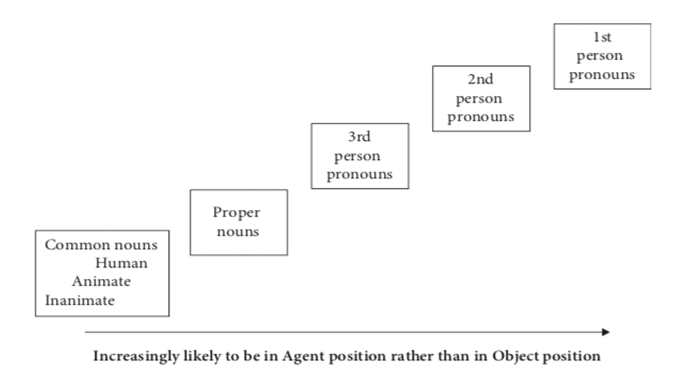
\includegraphics[width=16cm]{img/pronoun_animacy.png}
    \caption{Représentation des dénominations personnelles en fonction du degré d'\textit{animation} qu'elles évoquent - Ahearn (2001)}
    \label{pronoun_animacy}
\end{figure}

Là encore, la forme orale du théâtre rendait impossible l'utilisation de ce marqueur tel quel pour estimer l'agentivité du locuteur, puisque tous les personnages parlent à la première personne. Nous pouvions toutefois mesurer la proportion relative de pronoms à la première personne utilisés en position sujet, ou explicitement comme agents à la voix passive (en utilisant le \textit{parser} syntaxique de spaCy) dans chaque groupe de répliques, afin d’approximer très grossièrement leur agentivité grammaticale respective.

Pour la suite de l'analyse, et compte tenu de cette approximation très imparfaite, nous ne nous sommes pas limités à l'analyse des seules clauses dites « agentives » (celles comprenant un Agent au sens grammatical ou sémantique), mais nous avons plutôt dupliqué la mesure des indicateurs pour lesquels il était particulièrement difficile de savoir si leur relation avec l'agentivité dépendait du fait que le locuteur soit ou non le sujet de la clause, de la même façon que pour les verbes modaux. Nous avons ainsi dupliqué les mesures suivantes : verbes, copules, ratio de l'utilisation de la voix active vs. passive.

A titre de remarque, la gradation mentionnée ci-dessus a encore été utilisée dans l'analyse de la télicité : un personnage plus agentif pourrait en effet également être amené à prêter plus d'agentivité aux autres personnages qu'il ou elle mentionne, et ainsi à utiliser relativement plus de pronoms dénotant une animation particulière y compris lorsqu'il ou elle se réfère à d'autres individus. Il semble de fait qu'il existe un biais cognitif généralisé favorisant l'interprétation télique d'une phrase lorsqu'elle contient un sujet animé, et inversement une interprétation atélique dans le cas d'un sujet inanimé\footnote{\cite{graf_interaction_2017} - il s'agit là d'une études psycholinguistique, et non simplement théorique}. De manière cohérente, de nombreuses recherches indiquent que les entités inanimées sont incompatibles (ou du moins relativement moins compatibles que les entités animées) avec les verbes qui connotent l'intentionnalité, la planification ou impliquent des processus cognitifs, car ces entités inanimées n'ont pas les moyens de mener à bien des actions intentionnelles (voir ci-après).

\subsection{Voix active vs. passive}

Dans le même ordre d'idée, bien que cette fois-ci non soutenue par des travaux antérieurs, l'utilisation d'une voix active plutôt que passive (et malgré l'agentivité grammaticale qu'implique cette dernière) nous a semblé devoir être corrélée avec un degré d'agentivité plus élevé\footnote{\cite{hopper_transitivity_1980}}.

\subsection{Verbes statifs}

Un type de verbe pourrait constituer une exception univoque au lien verbe-agentivité : les verbes statifs ou d'état, qui se réfèrent principalement aux états émotionnels (et potentiellement durables) des agents, plutôt qu'à des actions. Il est vrai que l'on peut considérer les verbes exprimant des attitudes et des sentiments propositionnels comme évoquant des formes d'action mentale. Cependant, les \textit{verba sentiendi} (verbes de perception) sont généralement considérés comme moins « actifs ». 
Une autre composante linguistique de notre indice agentif a donc consisté à comparer la proportion relative de verbes purement statifs (ici approximés par l’utilisation des verbes \textit{être} et \textit{avoir} en excluant les emplois temporels, ainsi que par l'étiquette « copule » du \textit{parser} spaCy, les deux métriques étant mesurées séparément) par rapport aux verbes dits « dynamiques » (tous les autres verbes).

En guise de commentaire, et malgré leur supposée « stativité », l'utilisation du progressif avec des verbes d'émotions comme \textit{aimer} (par opposition à \textit{savoir}) semble en réalité être de plus en plus autorisée dans le langage courant, au moins à partir du XIX\ieme ~siècle pour l’anglais\footnote{\cite{granath_im_2014}}. Par ailleurs, Granath et al. notent qu'une telle combinaison entraînerait un changement aspectuel, suggérant alors une « agentivité accrue ». Cela remet en cause l'idée même d'une séparation binaire entre verbes statifs et non statifs, ces derniers se plaçant plutôt sur un continuum. De la même façon en effet, certains verbes appartenant traditionnellement à la catégorie des verbes dynamiques, notamment en référence à des activités et des événements physiques, se produisent rarement avec l'aspect progressif (par exemple \textit{shrug}, \textit{smash}, \textit{suck} et \textit{throw} en anglais). Notre analyse binaire est donc limitée, mais une approche tripartite, voire par degré de stativité, nécessitait de recourir à de la modélisation\footnote{\cite{klavans_degrees_1992}}\footnote{\cite{friedrich_automatic_2014}}\footnote{\cite{sims_literary_2019}}, ce qui dépassait le cadre technique de cette analyse. Aussi, nous avons tout de même mesuré l'usage relatif du progressif, considéré comme une indication potentiellement plus fine que l'opposition verbes statifs/autres verbes du dynamisme connoté par les événements, et indirectement de l'agentivité du locuteur (comparez simplement « je mange » avec « je suis en train de manger »).

\subsection{Transitivité}

Comme mentionné plus haut (I.2.1. \textit{Transitivité et foregrounding : des indices corrélés de l'efficacité de l'action}), la transitivité semble assez intuitivement liée à une perspective plus agentive, dans la mesure où le locuteur conçoit la possibilité d'une action directe sur un objet (grammatical). Une mesure de la proportion relative des verbes utilisés transitivement, plus proches de notre prototype de causalité\footnote{\cite{konopasky_towards_2016}}, a donc logiquement été ajoutée à notre indice.

\chapter{Traverser les distances psychologiques : l’agentivité et la planification}

Les gens sont capables de penser à l'avenir, au passé, à des endroits éloignés, à la perspective d'une autre personne et à des alternatives contrefactuelles. Sans nier le caractère unique de chaque processus, Trope et al.\footnote{\cite{trope_construal-level_2010}} ont proposé qu'ils constituent des formes différentes de franchissement d'une certaine distance psychologique. Selon eux, la distance psychologique est égocentrique : son point de référence est le soi, ici et maintenant (voir sur ce point la partie \textit{III. 2.2. Pronoms et déictiques : la référence au soi}), et les différentes façons dont un objet peut être éloigné de ce point (dans le temps, dans l'espace, dans la distance sociale et dans l'hypothéticité) constituent différentes dimensions de la distance. 

Aussi, plus les événements sont éloignés de l'expérience directe, plus ils sont susceptibles d'être représentés en des termes abstraits traduisant l'essence perçue des événements (constructions de haut niveau), plutôt qu'à travers les détails plus concrets et accessoires des événements (constructions de bas niveau), ce qui correspond étroitement à notre définition du continuum agentif. Cela est d'ailleurs corroboré par l’association, trouvée chez Woike\footnote{\cite{woike_use_1994}}, entre agentivité et différenciation (qui s'oppose au processus cognitif d’intégration\footnote{Les termes « séparé » et « connecté » ont souvent été utilisés pour décrire
deux conceptions différentes de l'individu par rapport au monde social : l'une comme autonome, indépendante et séparée des autres, et l'autre comme relationnelle, interdépendante et indépendante des autres. Pour Woike, cela suggère qu'il existe des processus cognitifs spécifiques impliqués dans la promotion et le maintien de ces deux orientations : la différenciation, qui consiste à percevoir un certain nombre d'aspects différents dans un groupe de stimuli donné, et l'intégration, qui consiste à établir des connexions ou des liens entre des stimuli différenciés}) : 

\begin{displayquote}
 « Parce que la différenciation implique de percevoir des différences et l'indépendance entre les attributs des stimuli sociaux, elle peut être utilisée plus fréquemment par les personnes qui ont une orientation vers l'individualisme et l'indépendance, car elle remplit une fonction particulière pour elles. Par exemple, Belenky et al. (1986) ont suggéré que la distance psychologique peut être maintenue en séparant le soi des objets sociaux afin de percevoir les choses de manière objective ou comme n'ayant aucun rapport avec soi. En outre, la pensée critique et la prise de décision sont, par définition, des procédures de comparaison qui impliquent de voir les différences relatives entre les choses. L'acte de séparer une question en la décomposant en plusieurs parties et en percevant ses contrastes et ses distinctions peut aider les percepteurs à porter des jugements et à prendre des décisions en limitant leur implication personnelle dans le contexte interpersonnel, ce qui leur permet de conserver une orientation individualiste. »
\end{displayquote}

Le degré de planification ou de capacité rétrospective de l'agent évoqués par une clause est ainsi une autre caractéristique linguistique importante.

\section{L’analyse aspectuelle de la télicité}

La télicité, ou « délimitation aspectuelle », est la propriété aspectuelle d'une phrase verbale (ou de la phrase dans son ensemble) qui indique qu'une action ou un événement a une fin spécifique. Du grec \textit{telos}, elle désigne plus précisément la « présence d'une finalité, intrinsèque ou envisagée, inhérente à l'événement, qui se manifeste mutuellement dès le moment où la situation a commencé et est évoquée », et au-delà de laquelle l'événement ne peut plus se poursuivre\footnote{\cite{depraetere_telicity_2007}}. A titre d’exemple, « courir vers quelqu'un » est considéré comme ayant un aspect plus télique que « jouer dans l'herbe » ou encore « marcher près d'un lac ».

Par définition, la télicité est donc liée à l'intentionnalité de l'agent. La manière dont un événement est évoqué (et réciproquement interprété) comme étant doté d'une valeur aspectuelle plus ou moins télique peut donc nous informer en partie quant à la mesure dans laquelle le locuteur se représente lui-même, ou ses \textit{alter ego}, comme capable d'agir volontairement sur le monde, par opposition à une idéologie plus fataliste par exemple. La télicité a donc également avoir, et ce d'une manière encore plus structurelle et compositionnelle, avec la notion d’agentivité. 

En nous inspirant de modèles d'apprentissage automatique de la télicité d'une clause (cités ci-après), qui donnaient accès aux principales caractéristiques utilisées par l'algorithme de classification (et dont la pertinence pour un lecteur humain était systématiquement vérifiée par la théorie linguistique ou par des études psycholinguistiques ultérieures), nous avons défini un certain nombre d'éléments linguistiques qui semblaient être décisifs dans la détermination de la télicité d'une phrase. Cette fois, et contrairement à la modalité, l'analyse se fait au niveau de la phrase-même (voire de la clause), puisque la télicité est définie de manière intrinsèquement compositionnelle (de telle sorte qu'une approximation au niveau des répliques concaténées des personnages n’avait pour le coup pas grand sens). En effet, si elle va souvent de pair avec les prédicats de réalisation et d'accomplissement, pour reprendre la classification de Vendler\footnote{\cite{vendler_verbs_nodate}: Les activités et les accomplissements se distinguent des réalisations et des états dans la mesure où les deux premières permettent l'utilisation d'aspects continus et progressifs. Les activités et les accomplissements se distinguent les unes des autres par leur délimitation. Les activités n'ont pas de point final (un point avant lequel l'activité a eu lieu et après lequel elle ne peut plus continuer, comme pour « Jean a dessiné un cercle »), alors que les accomplissements en ont un. En ce qui concerne les réalisations et les états, les réalisations sont instantanées, mais les états sont durables. Les réalisations et les accomplissements se distinguent l'un de l'autre par le fait que les réalisations ont lieu immédiatement (comme dans « reconnaître » ou « trouver »), alors que les accomplissements s'approchent progressivement d'un point final (comme dans « peindre un tableau » ou « construire une maison »).}, et s’il semble assez difficile d'exprimer un événement télique avec un prédicat de type activité ou état, les premiers ne peuvent garantir la télicité d'un événement.

En anglais comme en français, la télicité (un aspect interne) n'est pas non plus représentée par un marquage morphologique, contrairement à l'aspect externe (par exemple le progressif), bien qu'une corrélation ait été établie entre télicité et aspect parfait d'une part, et atélicité et progressif d'autre part\footnote{\cite{frawley_linguistic_1992}: cette étude est purement théorique}.

Il existe cependant certains critères qui détermineraient automatiquement la télicité d'une clause, et qui constituent donc des tests de télicité souvent mentionnés dans les articles théoriques. Notamment, le test de l'adverbe de temps demande si une phrase verbale est compatible avec le syntagme prépositionnel « dans un temps X » (télique) ou « pendant un temps X » (atélique). Un autre test fréquemment cité est celui de la compatibilité de la clause avec un adverbe d'intention tel que \textit{volontairement}.

Concrètement, nous avons donc défini un score « télique » pour chaque phrase, variant entre 0 (score initial) et 1 (phrase univoquement télique). Sur cette base, notre code teste tout d'abord la présence des marqueurs « automatiques » suivants au niveau de la phrase (nous n'avons en réalité pas été en mesure d'effectuer une décomposition syntaxique au niveau de la clause \textit{per se}, mais cette dernière est approximée par la présence d'un verbe, comme expliqué ci-après).

Notons qu'une fois encore, nous avons tenté de ne retenir que les déterminants les plus structurels (non sémantiques) pour conclure à la télicité d'une phrase, afin de contrôler autant que possible pour un biais d'interprétation moderne, qui pourrait voir un aspect télique dans des formes lexicales qui n'en évoquaient en réalité aucun chez les lecteurs contemporains de l'œuvre (le degré d'agentivité étant précisément censé s'accroître avec le temps). 

Les critères automatiques sont donc les suivants : 
a) « en X temps », qui rend la phrase systématiquement télique et fixe son score à 1 ; et « pendant X temps », qui la rend atélique et fixe son score final à 0. 

b) la présence d'un adverbe intentionnel (critère d'ailleurs limité dans son application, puisque le nombre d'adverbes univoquement volitifs est restreint), auquel cas le score phrastique est égal à 1 (voir la section I.1.2. \textit{Les adverbes intentionnels, statut hybride ?}).

c) un ajout personnel, mais étroitement lié au test d'intentionnalité présenté ci-dessus : les expressions de but (dont nous avons dressé une liste aussi exhaustive que possible, de la même manière que pour les adverbes intentionnels), pour lesquelles la présence d'au moins une expression fixe également le score à 1.

\begin{table}[ht]
\caption{Expressions à valeur de but retenues}
\centering
\bigskip
\renewcommand{\arraystretch}{1.5} % Adjust the value as needed
\begin{tabular}{|p{0.8\linewidth}|}
    \hline
    « pour », « finalité », « afin de/que », « à dessein de », « dans l’objectif/le but/l’intention/le dessein de », « de façon à/de cette façon/de telle façon que », « histoire de/que », « à la (seule) fin de »  \\
    \hline
\end{tabular}
 \label{Tab:adv_but}
\end{table}
\bigskip

Si la phrase contient au moins l’un de ces marqueurs, en considérant \textit{ a priori} comme marginaux les cas de combinaisons contradictoires entre ces derniers (quant à leur évocation télique ou atélique), l'analyse s'arrête ici pour la phrase en question, et le code nous fait passer à la suivante.

Si la phrase ne contient pas de tels critères « automatiques », le score de la phrase reste à 0, et l'analyse passe à un niveau plus fin : le code s'exécute pour chaque verbe de la phrase (et l'arborescence syntaxique de spaCy est telle qu'il n'était pas possible de limiter l'analyse aux verbes étiquetés comme « ROOT », sans perdre une partie de l'information qui nous intéressait pour la télicité). Tous les verbes sont donc analysés, y compris les verbes à l'infinitif qui dépendent d'un verbe conjugué (dans ce cas, certaines étiquettes de dépendance intéressantes sont associées au verbe à l'infinitif en question, et non au « ROOT »). Le code ajoute ensuite +1, ou respectivement -1, au score de télicité du semblant de clause (à savoir du verbe en question), également initialisé à 0, chaque fois qu'il rencontre l'un des marqueurs linguistiques suivants, sélectionnant une interprétation télique ou atélique : 

1. Comme mentionné ci-dessus, un temps parfait sélectionnerait une interprétation télique. Compte tenu des étiquettes disponibles, nous avons inclus le passé simple (présente dans le modèle fr de pie-extended) et le passé composé (identifié par la présence d'un auxiliaire de temps qui fait partie des étiquettes spaCy), en considérant qu’il s’agissait dans tous les cas d'un événement passé, à savoir terminé d'une manière ou d'une autre. Ces derniers ajoutent donc 1 au score clausal. A l'inverse, l'imparfait (étiquette du modèle fr) et le progressif (identifiée par l'expression régulière « en train de ») sélectionneraient une interprétation atélique, et réduisent ainsi le score de 1.

2. Alors que les phrases atéliques peuvent être intransitives ou avoir un objet direct optionnel qui modifie le prédicat, les phrases télique requièrent un participant à l'événement projeté en position d'objet (qui peut être réalisé comme un objet direct quantifié ou comme le sujet dans une construction non-accusative). La présence d'un objet grammatical (étiquette spaCy) ajoute donc 1 au score clausal.

3. En particulier, un objet quantifié (article défini, numéral) ou un objet dénombrable (\textit{count nouns} en anglais) nous obligent souvent à dériver une interprétation télique et, inversement, un objet indénombrable une interprétation atélique (\textit{mass nouns}). La présence d'un article défini ou numéral devant l'objet ajoute donc 1 au score clausal.

4. Selon Krifka\footnote{\cite{rothstein_what_nodate}}, la pluralité de l'objet direct signifie que l'événement doit être associé à une pluralité d'événements « en cours de réalisation », dont le nombre n'est pas précisé. De même, le point final de l'accomplissement est déterminé par le moment où le point final de tous ces événements est atteint, mais rien n'est dit sur leur nombre ni sur le fait qu'ils aient lieu simultanément ou séquentiellement. La localisation du point final dans le cas des « pluriels nus » (\textit{bare plurals} en anglais) n'est donc pas identifiable, et ils sélectionnent pour l'atélicité. La présence du pluriel indéfini \textit{des} devant l'objet, équivalent français le plus proche à nos yeux, soustrait donc 1 au score clausal.

Ajout personnel, mais qui nous a semblé intuitivement participer à l'individuation de l'objet grammatical en question : la présence d'un complément d'objet de tout type (adjectif, locution possessive [objet] de X etc.) associé à l'objet ajoute 1 au score clausal (concrètement, une étiquette spaCy « amod », « nod », « nmod » ou « appos » dans les dépendances syntaxiques de l'objet considéré). 

5. Une phrase prépositionnelle (PP) directionnelle peut également affecter la télicité : alors qu'un prédicat d'activité ne permet normalement pas l'interprétation télique, l'ajout d'une PP directionnelle peut contribuer à l'interprétation télique. En particulier (mais valant uniquement pour l'anglais ici, bien que nous réfléchissions plus tard à la possibilité d'un équivalent français), Walková\footnote{\cite{walkova_particle_2017}} distingue scalarité et télicité. Elle considère que la scalarité est une condition nécessaire mais non suffisante pour que l'effet de marquage de la télicité se produise. Ce qui compte vraiment, c'est en réalité que l'échelle en question soit bornée (verbes ou syntagmes téliques) ou non (atéliques). Atteindre la limite de l'échelle (notons qu'elle inclut dans son analyse les échelles à 2 points sous-jacentes aux événements ponctuels, qui eux sont toujours limités) équivaut à atteindre le point final de l'événement (c'est pourquoi la télicité est définie comme un point final temporel), bien que l'événement puisse en principe se poursuivre avec ce dernier type de limite.

Ainsi, les « particules scalaires » (celles qui peuvent affecter la structure argumentale de la racine du verbe et renforcer la télicité - \textit{down}, \textit{off}, \textit{out}, \textit{over}, \textit{through} et \textit{up} en anglais) marquent la télicité lorsqu'elles se réfèrent à une échelle lexicalisée dans un objet direct qui ne peut pas devenir un sujet non-accusatif.

Plus précisément, les particules scalaires ne peuvent apparaître qu'avec un objet direct quantifié. Lorsque la quantité est univoque (déterminant cardinal), elles renforceraient une sorte de télicité redondante ; et pour les syntagmes définis et possessifs (quantité ambiguë), elles imposeraient la télicité. Inversement, s'il n'y a pas d'autre constituant syntaxique « +scalaire », les « particules non-scalaires » (\textit{about}, \textit{along}, \textit{around}, \textit{on}, \textit{away}) n'affecteraient pas la structure argumentale du verbe, de sorte qu'elles ne pourraient renforcer la télicité. De manière cohérente, elles semblent même ajouter, dans ce cas, un sens qui pourrait être interprété comme dénotant un niveau inférieur d’agentivité (l'action étant vécue comme non intentionnelle et/ou intéressante en elle-même, dans son déroulement, plutôt que pour son résultat - pour reprendre la distinction souvent évoquée en linguistique entre \textit{path} et \textit{manner}).

Ainsi, et en considérant pour notre propos la possibilité d'une équivalence en français, les « verbes à particule » (à savoir ici les verbes suivis d'une préposition introduisant une construction verbale subordonnée) ajoutent 1 au score clausal. 

Autre initiative personnelle : si la préposition en question véhicule sémantiquement l'idée de direction (« jusque » et « vers » - à l'exclusion de leur utilisation dans des locutions adverbiales temporelles pour éviter la redondance avec ce qui suit), elle ajoute 1 au score clausal. Nous avons au passage dupliqué cette métrique, en comptant séparément le nombre relatif de prépositions directionnelles (\textit{jusque}, \textit{vers} ) et de manière ( \textit{par}, \textit{avec}, \textit{sans}) dans l'ensemble des répliques concaténées par statut (en les standardisant par le nombre total de mots et le nombre total de prépositions).

6. Depraetere\footnote{\cite{depraetere_telicity_2007}} suggère également (et c'est sa définition de la télicité que nous avons citée en introduction, car elle était la plus pertinente pour notre question de recherche) que l'intentionnalité est nécessaire à la télicité. Selon elle, certains types de constituants quantifiés (phrases nominales, numériques, et adverbiaux) ne seront associés à la fonction de fin inhérente que s'ils sont « dans l'horizon » d'une intention mutuellement manifeste. L'intentionnalité est donc une propriété \textit{a priori} exclusive des sujets animés. La présence d'un pronom sujet ou d'un nom propre ajoute ainsi 1 au score clausal.

7. Une corrélation entre la télicité et la voix passive a également été établie par Frawley\footnote{\cite{frawley_linguistic_1992}}. Ce dernier soutient que la logique du passif étant de « promouvoir le destinataire de l'action à la position de sujet », il mettrait l'accent sur le résultat du processus encodé par le verbe dans la mesure où le destinataire est le résultat de l'action, produisant ainsi une interprétation télique. Pour autant, nous considérons plutôt que la voix active est la plus à même de renforcer la télicité d'une clause (en renforçant la transitivité du verbe, par souci de cohérence avec ce dernier critère). La présence d'une construction passive (donnée par spaCy) soustrait donc 1 au score clausal.

8. Les modèles d'apprentissage automatique récemment développés pour déterminer la télicité des clauses\footnote{\cite{siegel_learning_2000}}\footnote{\cite{zarcone_computational_2008}}\footnote{\cite{friedrich_classification_2017}}\footnote{\cite{zhao_pretrained_2021}} confirment les marqueurs mentionnés ci-dessus, à savoir que les transformateurs y prêtent également attention lorsqu'ils concluent sur la télicité des clauses. Ces modèles nous ont encore permis d'ajouter un critère adverbial, les études en question ayant montré qu'il était également valable pour l'interprétation aspectuelle des participants humains. Nous avons donc construit en amont des listes d'adverbes temporels, locatifs et de manière, à partir du croisement de plusieurs grammaires françaises. Nous avons également dressé une liste, aussi exhaustive que possible, des expressions temporelles pouvant être utilisées pour construire des compléments à valeur adverbiale temporelle ( \textit{heures}, \textit{minutes}, etc.), en localisant leur occurrence à des positions syntaxiques spécifiques qui devraient le plus souvent correspondre à une telle valeur.

\begin{table}[H]
\caption{Expressions adverbiales de manière retenues}
\centering
\bigskip
\renewcommand{\arraystretch}{1.5} % Adjust the value as needed
\begin{tabular}{|p{0.8\linewidth}|}
    \hline
    « à bras-le-corps », « à califourchon », « à la légère », « à la va-comme-je-te-pousse », « à la va-vite », « à l'aveuglette », « à loisir », « à nouveau », « de nouveau », « à tire-d'aile », « à tire-larigot », « à tort », « à tue-tête », « bel et bien », « bon marché », « d'arrache-pied », « de guingois », « par hasard », « pour de bon », « tant bien que mal », « comme », « comment », « ainsi », « aussi », « bien », « debout », « également », « ensemble », « franco », « gratis », « incognito », « mal », « mieux », « pis », « plutôt », « presque », « quasi », « recta », « vite », « volontiers »  \\
    \hline
\end{tabular}
 \label{Tab:adv_maniere}
\end{table}

\begin{table}[H]
\caption{Expressions adverbiales de lieu retenues}
\centering
\bigskip
\renewcommand{\arraystretch}{1.5} % Adjust the value as needed
\begin{tabular}{|p{0.8\linewidth}|}
    \hline
    « à proximité », « aí », « aux abords de », « aux abords du », « aux abords d », « ailleurs », « alentour », « alentours », « arrière », « attenant », « au diable Vauvert », « autour », « en bas », « vers », « çà », « céans », « chez », « ci », « à côté », « sur le côté », « au côté », « deçà », « delà », « dedans », « dehors », « derrière », « dessous », « dessus », « devant », « à droite », « à gauche », « exa », « à l'extérieur », « face à », « face au », « hái », « en haut », « ici », « là », « à l'intérieur », « léans », « loin », « nulle part », « où », « par monts et par vaux », « partout », « près de », « près du », « près d », « proche de », « proche du », « proche d », « quelque part », « sus », « y »  \\
    \hline
\end{tabular}
 \label{Tab:adv_loca}
\end{table}

\begin{table}[H]
\caption{Expressions adverbiales temporelles retenues}
\centering
\bigskip
\renewcommand{\arraystretch}{1.5} % Adjust the value as needed
\begin{tabular}{|p{0.8\linewidth}|}
    \hline
    « à présent », « a présent », « à l'approche d », « a l'approche d », « à l'approche de », « a l'approche de », « à l'approche du », « a l'approche du », « à l'approche des », « a l'approche des », « sur le moment », « sur l'heure », « un temps », « un moment », « un instant », « un jour », « un matin », « une nuit », « un soir », « une soirée », « un beau jour », « un beau matin », « un beau soir », « un hiver », « un été », « un printemps », « un automne », « une année », « d'un moment à l'autre », « d'un instant à l'autre », « un de ces jours », « au début », « au commencement », « à la fin », « a la fin », « en fin », « au milieu », « aux environs de », « aux environs d », « actuellement », « anciennement », « simultanément », « de jour », « de nuit », « en simultané », « fréquemment », « régulièrement », « antan », « après », « alors », « auparavant », « aussitôt », « autrefois », « avant », « bientôt », « dans peu », « de suite », « de ce pas », « de temps en temps », « déjà », « demain », « d’main », « depuis », « derechef », « dernièrement », « désormais », « de tout temps », « de tous temps », « d'abord », « dorénavant », « encore », « enfin », « ensuite », « entre-temps », « entretemps », « quelque temps », « hier », « hui », « illico », « immédiatement », « instantanément », « sous peu », « jadis », « jamais », « jusqu'à », « jusqu'au », « jusqu'aux », « jusque », « longtemps », « lors », « maintenant », « maishui », « meshui », « méshui », « momentanément », « naguère », « naguères », « parfois », « présentement », « prochainement », « puis », « quelquefois », « rarement », « récemment », « sans délai », « sans perdre un instant », « sans attendre », « sans tarder », « sans trop tarder », « sitôt », « soudain », « soudainement », « souvent », « subito », « sur-le-champ », « sur le champ », « sur le coup », « sur le coup de », « sur les coups de », « tantôt », « tard », « tardivement », « tôt », « toujours », « tout à coup » ,« tout d'un coup », « tout le long de », « tout le long du », « tout le long d », « tu suite », « tandis », « quand », « lorsque », « lorsqu », « une fois que », « une fois qu », « pendant que », « pendant qu », « cependant que », « cependant qu », « chaque fois que », « chaque fois qu », « toutes les fois que », « toutes les fois qu », « tant que », « tant qu », « à mesure », « a mesure », « le temps que », « le temps qu », « dès », « en attendant », « le temps de », « le temps d », « le temps du », « durant », « pendant », « au cours de », « au cours d », « l'espace d'un instant », « dans l'instant », « au bout d », « au bout de », « à partir de », « à partir d », « lundi », « mardi », « mercredi », « jeudi », « vendredi »,  « samedi », « dimanche », « piéça » \\
    \hline
\end{tabular}
 \label{Tab:adv_temp}
\end{table}

\begin{table}[H]
\caption{Lexique univoquement temporel retenu en complément des expressions adverbiales précédentes pour l'analyse regex}
\centering
\bigskip
\renewcommand{\arraystretch}{1.5} % Adjust the value as needed
\begin{tabular}{|p{0.8\linewidth}|}
    \hline
    « coucher », « lever », « an », « ans », « année », « années », « soir », « soirs », « soirée », « soirées », « matin », « matins », « matinée », « matinées », « jour », « jours », « nuit », « nuits », « journée », « journées », « midi », « midis », « minuit », « heure », « heures », « minute », « minutes », « seconde », « secondes », « mois », « janvier », « février », « mars », « avril », « mai », « juin », « juillet », « août », « septembre », « octobre », « novembre », « décembre », « siècle », « siècles », « saison », « saisons », « hiver », « printemps », « été », « automne », « étés », « hivers », « printemps », « automnes », « semaine », « semaines », « temps », « moment », « moments », « instant », « instants », « fois » \\
    \hline
\end{tabular}
 \label{Tab:adv_temp_bis}
\end{table}

Finalement, le score de la clause (c.a.d. de chaque verbe étudié) a été normalisé, suivi du score de la phrase (la normalisation prenant comme paramètre le nombre de clauses présentes dans la phrase en question, qui détermine les scores maximum et minimum utilisés pour la normalisation) et du score total du texte, calculé en faisant la moyenne des scores de toutes les phrases analysées.

\subsection{Les modes de l’irréel et la pensée hypothétique}

Les modes de l’irréel font référence à l'ensemble des modes grammaticaux indiquant qu'une certaine situation ou action n'est pas connue pour s'être produite au moment où le locuteur parle. Sur la base de la classification de Wikipedia (valable pour l'anglais et le français)\footnote{\url{https://fr.wikipedia.org/wiki/Mode_(grammaire)}}, nous avons ainsi mesuré la proportion relative des formes indicatives par rapport aux formes non affirmatives (subjonctif, conditionnel, interrogatif et impératif). 

Comme mentionné précédemment, nous avons encore mesuré l'utilisation du futur, en considérant qu'il dénotait également une modalité épistémique irréelle.

Enfin, nous avons quantifié la fréquence d'alternance entre les temps pour les personnages de haut et de bas statut, en supposant qu'une plus grande capacité de distanciation psychologique devrait se traduire, en moyenne, par des allers-retours plus fréquents entre des considérations rétrospectives, présentes et anticipatrices.

\subsection{Les marqueurs corrélés d’abstraction}

Dans son article de 2021, Lievers\footnote{\cite{strik_lievers_linguistic_2021}} énumère une panoplie de marqueurs linguistiques qui peuvent être utilisés comme proxys pour estimer le niveau d'abstraction d'un texte, sans avoir à mobiliser un modèle d'apprentissage particulièrement complexe pour cette tâche. Parmi tous ceux qu'il propose, le plus facile à mettre en œuvre était la fréquence relative d'utilisation des parties du discours principalement associées à un sens plus abstrait (à savoir les adverbes ; les \textit{mots-outils}, c.a.d. les déterminants et adjectifs non qualificatifs, conjonctions, prépositions excluant les locatifs, pronoms, auxiliaires, modaux, outils interrogatifs, qualificatifs ; et les adjectifs), par rapport à ceux associés à un sens plus concret (noms et verbes). 

Comme on l’a expliqué, cet indicateur implique une incertitude quant à la direction de la corrélation attendue pour le nombre de verbes utilisés par chaque groupe de personnages, les verbes étant intuitivement liés à l’agentivité dans le sens d’une plus grande disposition à agir, réalisée ou non, mais inversement corrélés si l'on considère le niveau d'abstraction supplémentaire que les agents « haut niveau » sont censés mobiliser. C'est ce qui motive l'utilisation d'un indice agentif global, qui devrait résister à de telles ambiguïtés individuelles.

\chapter{Le langage de la personnalité : indices d’extraversion et d’agréabilité}

Une précision s'impose concernant l'analyse des marqueurs linguistiques associés respectivement à l'extraversion et à l'agréabilité, censés garantir la spécificité de notre indice agentif. 

En nous appuyant notamment sur les travaux de Pennebaker\footnote{\cite{pennebaker_linguistic_nodate};\cite{pennebaker_expressive_2007}}, qui a principalement utilisé le LIWC\footnote{Le LIWC consiste notamment en une collection de dictionnaires répertoriant les mots relatifs à des catégories sémantiques spécfiiques, et créés par les utilisateurs eux-mêmes : \url{https://www.liwc.app/}} pour ses études, bien qu'il ait également été en mesure d'identifier des associations linguistiques plus « structurelles » que nous avons déjà pris en compte, nous avons pu dresser la liste des indicateurs linguistiques ci-dessous\footnote{Pour une liste complète des références parcourues avant de parvenir à cette sélection : \cite{pennebaker_linguistic_nodate}; \cite{heylighen_variation_2002}; \cite{pennebaker_expressive_2007}; \cite{oberlander_whose_2006}; \cite{mairesse_using_2007}; \cite{gill_what_2009}; \cite{yarkoni_personality_2010}; \cite{chittaranjan_whos_2011}; \cite{kern_sooo_2014}; \cite{schwartz_personality_2013}; \cite{celli_pr2_2014}\cite{mehta_bottom-up_2020}; \cite{carducci_personality_2020}; \cite{stajner_survey_2020}} :

\begin{center}
\begin{table}[ht]
\renewcommand{\arraystretch}{1.8} % Adjust the value as needed
\caption{Récapitulatif des marqueurs linguistiques distinctifs identifiés pour les deux catégories de traits d'intérêt du modèle des \textit{Big Five}}
\bigskip
\begin{tabular}{ |p{9cm}|p{6cm}| }
 \hline
 \underline{Extraversion} \newline{(et Consciensiosité)} &  \underline{Agréabilité} \newline{(et Ouverture)} \\
 \hline
    Points d'interrogation (-) & Points d'interrogation (+) \\
    \underline{Articles (-)} & Articles (+) \\
    \underline{\textbf{Négations (-)}} & Passé (-) \\
    \underline{Style implicite (verbes, adverbes, pronoms) (+)} & \\
    \underline{Style formel (par opposition à contextuel) (-)} & \\
    \underline{Richesse lexicale (Uber index) (-)} & \\
    \underline{WPS (\small{\textit{words per sentence}}) (+)} \\
 \hline
\end{tabular}
\end{table}
    \label{Tab:recap_marqueurs_personnalite}
\end{center}

\vspace{-20pt} % Adjust the value to reduce the space

Les mots soulignés sont ceux dont l'utilisation a été directement associée aux deux traits les plus déterminants que sont l'extraversion et l'agréabilité dans la littérature (à savoir les traits les plus directement associés à l’agentivité et à la communion, respectivement). En gras, le marqueur a également été associé de manière cohérente au trait de caractère plus secondaire mentionné (respectivement la conscienciosité et l'ouverture). Le signe + ou - indique la corrélation positive ou négative attendue avec le trait de personnalité en question.

Concernant la ponctuation, nous avons ajouté, en plus des points d’interrogation, des métriques retraçant l’usage de tous les autres signes de ponctuation, certaines des études mentionnées laissant penser qu’il existerait là aussi des associations préférentielles selon la personnalité du locuteur, bien que ces signes n’étaient \textit{a priori} pas distinctifs s’agissant de la corrélation avec l’extraversion/consciosité et l’agréabilité/ouverture respectivement (à savoir qu’ils étaient corrélés à ces deux catégories de traits simultanément, et ce dans la même direction – par exemple positivement corrélés à la fois à l’extraversion et à l’agréabilité ; ou bien encore qu’ils étaient inversement corrélés à chacun des deux traits mentionnés au sein desdites catégories – par exemple positivement corrélés à l’agréabilité mais négativement corrélés à l’ouverture, ce qui limitait à première vue leur robustesse pour servir de marqueur distinctif). 

Pour la même raison, nous avons inclus dans nos métriques le comptage du nombre total de mots, de phrases, ainsi que des mots de plus de 6 lettres, tous étudiés en association avec la personnalité du locuteur mais se révélant, dans les études en question, non distinctifs.

La détermination de la formalité du style correspond au calcul de l'indice suivant : F = (fréquence du nom + fréquence de l'adjectif + fréquence de la préposition + fréquence de l'article - fréquence du pronom - fréquence du verbe - fréquence de l'adverbe - fréquence de l'interjection + 100)/2. Les personnes plus extraverties ont été identifiées comme utilisant un langage moins formel (et corollairement plus contextuel) que les personnes plus introverties.

Comme mentionné dans le tableau, un style de pensée plus implicite, caractérisant les individus plus extravertis, fait référence à l'utilisation relativement plus importante de verbes, d'adverbes et de pronoms, pour lesquels nous avons construit une métrique séparée, en plus du suivi individuel de ces différentes parties du discours.

Enfin, la richesse lexicale correspond au calcul de l'indice de « Uber » suivant : 
\begin{equation}
U = \frac{log(tokens)^2}{log(\textit{tokens}) - log(types)}
\end{equation}

 Les \textit{tokens} correspondent au nombre de mots (tels qu'identifiés par spaCy), et les \textit{types} au nombre de mots uniques ou distincts utilisés (à l'exclusion des \textit{mots-outils} ou de la ponctuation), le rapport des deux fournissant une approximation de la diversité lexicale des répliques d'un personnage. Nous avons également calculé, séparément, le ratio du nombre de \textit{tokens} différents utilisés par rapport au nombre total de mots, bien que ce marqueur ait été corrélé négativement à la fois à l’extraversion et à l’agréabilité.

De façon très exploratoire, nous avons également intégré dans notre code deux métriques s’attachant à approximer deux styles de pensée censés être relativement exclusifs : un style de pensée « catégorique », positivement corrélé avec le succès académique dans une étude menée par Pennebaker\footnote{\cite{pennebaker_when_2015}}, et dont la prévalence serait, à titre purement spéculatif, attendue chez les individus relativement plus agentifs (l'agentivité étant liée à l'assertivité, qui devrait logiquement se traduire par des réussites personnelles relativement plus nombreuses, y compris dans le domaine scolaire) ; et un style de pensée plus « dynamique », quant à lui corrélé négativement avec le succès académique et qui pourrait ainsi davantage caractériser les individus relativement moins agentifs. D’un point de vue linguistique, un style catégorique se traduit par l’utilisation d’articles, de prépositions, et dans une certaine mesure de conjonctions et de négations (bien que les résultats soient contradictoires pour ces deux derniers marqueurs) relativement plus fréquente. A l’inverse, un style de pensée dynamique ou « flexible » correspond à l’usage préférentiel de verbes auxiliaires, de pronoms et d’adverbes\footnote{\cite{chung_psychological_nodate}\footnote{\cite{pennebaker_when_2015}\footnote{\cite{dzogang_diurnal_2018}}.

Outre leur utilité pour la validation externe qui devra être menée ultérieurement, tous les marqueurs associés à l'extraversion ont été intégrés au calcul du score agentif discuté plus bas.
\part{Résultats et discussion}

\chapter{Des résultats prometteurs}

Pour construire notre indice global d’agentivité, calculé au niveau de chaque pièce, nous avons tout d'abord normalisé les mesures de chaque métrique linguistique afin qu’elles soient comprises entre 0 et 1. Nous avons ensuite additionné, pour une pièce considérée, le score de toutes les métriques calculées par statut (haut/bas) ou respectivement par genre (masculin/féminin), des personnages ayant prononcé les répliques concaténées, et sur la base desquelles chaque métrique avait été calculée dans la pièce en question. La somme obtenue correspond ainsi, pour chaque pièce, au score d’une  « méga-variable » calculée par statut (resp. par genre), et constituant la première ébauche de notre indice agentif. Ce score est compris entre 0 et 1.

Au total (en considérant toutes les pièces analysées dans notre corpus), nous disposons de 888 observations afin de tester l’association entre  « mégascore » agentif et statut des personnages, et de 891 observations s’agissant de l’association entre le mégascore agentif et le genre des personnages. 
A partir de tous ces points, nous tentons donc d’estimer la corrélation entre l'indice d’agentivité ainsi construit et la variable catégorielle \textit{statut} (resp. \textit{genre}), à l'aide de différents modèles de régression linéaire détaillés ci-après :

-Un modèle de régression simple calculant l’impact du Statut (resp. Genre) sur le mégascore agentif.

-Un modèle de régression logit calculant à l’inverse l’impact du mégascore agentif sur le Statut (resp. Genre) des personnages locuteurs.

A noter que pour l’analyse s’intéressant au statut, nous avons en réalité construit non pas deux mais quatre modèles de régression au total, en dupliquant chaque modèle selon que l’on prenait en compte, ou non, la direction de corrélation attendue (positive ou négative) pour chacune des métriques linguistiques avec le score agentif. On notera que les verbes sont comptés positivement ici, y compris les verbes modaux et l'usage de la modalité en général (en ce qu'elle reflète supposément une agentivité  « morale »), ce malgré l'ambiguïté mentionnée dans les sections correspondantes pour ces marqueurs. L'on considère en effet dans cette première ébauche que le verbe reste, intuitivement, un proto-marqueur agentif qu'il serait difficile d'ignorer, en sachant que si la direction s'avère contraire à celle prédite, cela ne devrait pas être suffisamment important pour affecter la direction du score global étant donnée la multitude d'autres métriques incluses dans son calcul. Et c'est en ce sens que nous conservons malgré tout un calcul plus  « grossier » du score agentif, qui somme simplement toutes les métriques dont on pense qu'elles ont avoir avec la notion d'agentivité, quelle que soit la direction de la corrélation postulée.
Nous avons également supprimé du calcul du score agentif, dans la seconde version des modèles, les métriques pour lesquelles la direction de corrélation demeurait trop ambigüe, à savoir : le nombre de parenthèses, points, virgules, points-virgules, deux points, guillemets, apostrophes, tirets et l'emploi du gérondif\footnote{Ces métriques n'ont d'ailleurs pas été mentionnées du tout, ou seulement très brièvement, dans le corps de ce mémoire. En guise de précision donc, les signes de ponctuation supprimés dans la seconde version des modèles étaient régulièrement associés à des traits de personnalité d'intérêt du \textit{Big Five} dans les études correspondantes parcourues, mais ce de façon contradictoire et \textit{a fortiori }non distinctive. Quant au gérondif, l'on avait supposé qu'il pourrait venir s'ajouter aux proxy téliques individuels - hors analyse compositionnelle, en ce qu'il dénoterait en l'occurrence un aspect atélique par la focalisation sur le déroulement de l'action qu'il sous-tend. Cela dit, cette interprétation demeurait très personnelle et incertaine, n'étant soutenue par aucune étude spécifique. Il est donc également supprimé du calcul du score dans la seconde version des modèles. On précisera enfin, au passage, que la suppression des métriques comptant le nombre de phrases et de mots prononcés dans le calcul de l'indice agentif ne change pas la significativité des résultats qui suivent, de sorte que cet indice ne se contente pas de révéler le fait qu'un maitre parle plus souvent, et/ou plus longtemps, que son serviteur dans la pièce, toutes les autres métriques incluses étant normalisées en fonction du nombre total de mots dans chacun des deux groupes de répliques précisément afin de prévenir ce biais.}.

Ce problème ne s’est pas posé concernant le genre, pour lequel nous n’avions pas de quoi supposer, \textit{a piriori}, une direction de corrélation précise pour chaque métrique de l’indice, par rapport au genre. Dans ce cas en effet, nous supposons simplement que le score agentif, même s'il comprend certaines métriques en réalité inversement corrélées à ce dernier et ayant donc un score plus faible quand ce degré d'agentivité augmente, devrait globalement corréler positivement avec le genre masculin, contrairement à celui féminin.

Concernant le statut des personnages tout d’abord, les résultats sont donc présentés ici respectivement sans et avec prise en compte des directions de corrélation propres à chaque métrique (à savoir que dans la seconde version de chacun des modèles, les métriques suivantes ont été comptées négativement au moment de calculer le mégascore agentif : ponctuation, ellipses, ratio du nombre de \textit{tokens} différents utilisés par rapport au nombre total de mots ou lemmes - deux versions d'une même métrique, indice de richesse lexicale, noms, articles, adverbes de manière, adverbes de doute, négations, présent, imparfait, indicatif, verbes statifs, copules, prépositions de manière, formalité, style  « dynamique »).

En moyenne, le mégascore agentif est de 23.5 pour les personnages de haut statut contre 22.5 pour ceux de bas statut (respectivement 7.35 contre 6.24 en prenant en compte les directions).

\begin{table}[ht]
\caption{Score agentif par statut - modèle 1}
\centering
\bigskip
\begin{tabular}{lS[table-format=2.1]S[table-format=1.3]}
    \hline
    Statut &  Moyenne & Ecart-type \\
    \hline
    Haut &  23.5 & 0.826 \\
    Bas &  22.5 & 1.22 \\
    \hline
\end{tabular}
 \label{Tab:moystatut}
\end{table}
\bigskip

\begin{table}[ht]
\caption{Score agentif par statut - modèle 2}
\centering
\bigskip
\begin{tabular}{lS[table-format=2.1]S[table-format=1.3]}
    \hline
    Statut &  Moyenne & Ecart-type \\
    \hline
    Haut &  7.35 & 0.940 \\
    Bas &  6.24 & 1.05 \\
    \hline
\end{tabular}
 \label{Tab:moy_statut}
\end{table}
\bigskip

Aussi, un t.test nous révèle que la différence de moyenne du mégascore agentif entre ces deux statuts est chaque fois significative (p < 0.001). 

En appliquant le modèle de régression linéaire simple suivant : 

\begin{equation}
\text{Score} \, \text{agentif} \, \sim \, \text{Statut}
\end{equation}

On trouve de façon cohérente qu’il existe une association linéaire significative entre le mégascore agentif et la variable catégorique \textit{statut}, ce avec et sans prise en compte des directions de corrélation individuelles (p < 0.001). 

D’après le premier modèle, le fait de passer de la catégorie  « bas » à  « haut » statut, toutes choses égales par ailleurs, augmente la valeur moyenne du score agentif de 1.01, contre 1.11 dans le second modèle.

Le $R^2$ pour chacun des deux modèles est de 0.19 et 0.24 respectivement, avec un sigma (écart-type du terme d’erreur) de 1.04 et 1. Le second modèle explique donc une plus grande proportion de la variance du score agentif, et génère des prédictions plus proches des points de données réels (sigma plus faible). Il peut ainsi être considéré comme ayant une meilleure adéquation aussi bien en termes de $R^2$ que de minimisation des erreurs de prédiction. 

Puisqu’il n’était pas aisé de savoir si l’on s’attendait à ce que le statut permette de prédire le langage utilisé dans la pièce, ou bien plutôt à ce que l’utilisation d’un certain langage prédise le statut des personnages, nous avons également analysé le modèle de régression logistique suivant : 

\begin{equation}
\text{Statut} \, \sim \, \text{Score} \, \text{agentif}
\end{equation}

Là encore, l’association est chaque fois très significative (p < 0.001), la seconde version du modèle (avec prise en compte des directions individuelles) présentant de façon cohérente un meilleur « fit » que la première (déviance résiduelle et AIC plus faible), ainsi qu'un coefficient de score agentif un peu plus élevé. 

Exprimé en ratio de vraisemblance (et non plus en logarithme de ce dernier), le premier modèle indique que pour chaque augmentation d’une unité du score agentif des répliques considérées, les chances que leurs locuteurs soient de haut statut sont 2.8 fois plus élevées, toutes choses égales par ailleurs (l’intervalle de confiance à 95\% associé étant : [2.29, 3.53]). Le second modèle (avec prise en compte des directions individuelles) présente quant à lui un odds-ratio de 3.03 ([2.49, 3.75]).

S’agissant des modèles logistiques, nous avons encore testé leurs performances prédictives au moyen d’une validation croisée dix fois. La précision de chacun des modèles (sans et avec prise en compte des direction de corrélation respectivement) est de 75\% et 79\% respectivement, leur sensibilité de 78\% et 77\%, et ainsi leur F1-score de 77\% et 78\%. Si le second modèle est légèrement plus précis que le premier (relativement moins de faux positifs), leurs performances prédictives globales sont donc équivalentes.

\begin{table}[ht]
  	\caption{Résultats de l'évaluation des modèles logistiques relatifs au statut en validation croisée}
		\centering % Centre the table on the slide
		\begin{tabular}{l c c c c c}
			\toprule
    			 & precision & recall & f1-score \\
			\toprule
			Modèle 1 & 0.754 & 0.782 & 0.768 \\
			\midrule
			Modèle 2 & 0.786 & 0.774 & 0.780 \\
			\bottomrule
		\end{tabular}
            \label{Tab:logit_statut}
	\end{table} 

Concernant le genre des personnages cette fois, pour lequel nous avons systématiquement conservé toutes les métriques sans duplication des modèles, on trouve qu’en moyenne, le mégascore agentif est de 29 pour les personnages féminins contre 29.1 pour les locuteurs masculins. Un t.test nous confirme que cette différence de moyenne du mégascore agentif entre les deux genres n’est pas du tout significative (p = 0.9921). 


\begin{table}[ht]
\caption{Score agentif par genre}
\centering
\bigskip
\begin{tabular}{lS[table-format=2.1]S[table-format=1.3]}
    \hline
    Genre &  Moyenne & Ecart-type \\
    \hline
    Masculin &  29.1 & 0.830 \\
    Féminin &  29.0 & 1.06 \\
    \hline
\end{tabular}
 \label{Tab:moy_genre}
\end{table}
\bigskip

En appliquant le modèle de régression linéaire simple suivant : 

\begin{equation}
\text{Score} \, \text{agentif} \, \sim \, \text{Genre}
\end{equation}

On trouve qu’il existe une association linéaire faiblement significative (p = 0.0159) entre ces deux variables que sont le mégascore agentif et genre du personnage. 

Le fait de passer de la catégorie « féminin » à « masculin » augmente plus précisément la valeur moyenne du score agentif de 0.15, toutes choses égales par ailleurs.

Le $R^2$ du modèle est de 0.007, et son sigma de 0.95. Cela suggère que le genre, en tant que seul prédicteur, n'explique pas une grande partie de la variabilité du mégascore agentif. Sa significativité pratique serait donc limitée. Les prédictions du modèle sont du reste relativement proches des points de données réels (sigma faible).

Pour les mêmes raisons que précédemment, nous avons également analysé le modèle de régression logistique suivant : 

\begin{equation}
\text{Genre} \, \sim \, \text{Score} \, \text{agentif}
\end{equation}

Là encore, l’association est faiblement significative (p = 0.0374).

Aussi, le modèle indique que pour chaque augmentation d’une unité du score agentif des répliques considérées, les chances que leurs locuteurs soient des personnages masculins sont 1.2 fois plus élevées, toutes choses égales par ailleurs (l’intervalle de confiance à 95\% associé étant : [1.01, 1.45]). 

Nous avons à nouveau testé ses performances prédictives au moyen d’une validation croisée dix fois. La précision du modèle est de 54\%, sa sensibilité de 52\%, et ainsi son F1-score de 53\%. Ce modèle est donc, logiquement, très peu performant lorsqu’il s’agit de prédire le genre du personnage locuteur, sur la base du mégascore agentif seul.

\begin{table}[ht]
\caption{Résultats de l'évaluation du modèle logistique relatif au genre en validation croisée}
		\centering % Centre the table on the slide
		\begin{tabular}{l c c c c c}
			\toprule
    			 & precision & recall & f1-score \\
			\toprule
			     & 0.539 & 0.512 & 0.529 \\
			\bottomrule
		\end{tabular}
            \label{Tab:logit_genre}
	\end{table} 

\bigskip
Ces résultats constituent donc une première confirmation de nos intuitions théoriques, à savoir que le niveau d'agentivité d'un personnage, tel que nous l'avons défini théoriquement et sur la base d'une validation interne à la pièce (c'est-à-dire a priori informés par le statut du personnage), semble être identifiable de manière relativement systématique par un ensemble de marqueurs linguistiques au niveau agrégé. 

Il est également rassurant que la seconde version de notre modèle linéaire simple s’attachant à expliquer le mégascore agentif par le statut du personnage se révèle globalement plus performant que la première. A savoir que la prise en compte des directions de corrélation propre à chaque marqueur linguistique rend de fait le niveau d’agentivité des locuteurs (approximé par leur statut) plus « capable » d’expliquer leur mégascore agentif, ainsi calculé.

Néanmoins, la première tentative de validation externe de notre indice agentif global, au moyen du genre des personnages, est pour sa part peu concluante. De fait, l’association entre genre et mégascore agentif n’est que très faiblement significative, et les performances prédictives d’un modèle de régression logistique tentant d’expliquer ledit mégascore par le genre des locuteurs sont à peine supérieures à celles qu’obtiendrait un modèle de classification aléatoire. 

Cela étant, la notion de genre ne se limite pas à l’agentivité, et est susceptible de charrier un certain nombre d’autres dimensions qui pourraient précisément interférer avec le degré d’agentivité d’un individu au moment de façonner son langage. Il n’est donc pas étonnant que la corrélation soit moins évidente que pour le statut. Ce d'autant plus que, n'ayant pas eu le temps de nous plonger dans la littérature s'intéressant aux associations préférentielles entre genre et langage, nous n'avons pas entrepris d'affiner le calcul de notre indice par la prise en compte de la direction de corrélation précise attendue pour chaque métrique prise isolément (et il semblait peu justifié, à ce stade, de simplement répliquer les directions de corrélation prédites pour le statut et non pour le genre spécifiquement). Aussi, on notera que la direction globale prédite est quant à elle respectée, à savoir que l’indice agentif est bien préférentiellement associé au genre masculin, bien que cette préférence soit légère, par rapport à celui féminin.

\chapter{Discussion}

\section{Limites de la présente recherche}

Notre étude, très exploratoire, connait bien entendu certaines limites. 

Tout d’abord, un certain nombre de travaux sur lesquels nous nous appuyons afin de définir, \textit{a priori}, nos marqueurs linguistiques agentifs ne triangulent pas les données en faisant notamment appel, outre l'analyse de corpus par  « lecture distante », à des expériences psycholinguistiques. Certains marqueurs sont donc étiquetés agentifs sur la base de la seule appréciation subjective de l’auteur, et certains résultats sont d’ailleurs en partie mis en cause par des études contradictoires (pour la modalité notamment). 

Aussi, toutes ces études valent pour l’anglais et non le français. Pour autant, notre recherche s’intéressant en priorité à des marqueurs  « structurels » (c.a.d. aux niveaux grammatical et syntaxique) relativement simples, la transposition des conclusions au français ne nous semblait pas déraisonnable (la présence d’un objet grammatical par exemple, semble devoir produire un effet relativement similaire quelle que soit la langue considérée, d’autant plus entre des locuteurs appartenant à des sociétés culturellement proches comme le sont les Etats-Unis et la France). Nous sommes toutefois conscients qu'il existe des différences notables entre ces deux langues, s’agissant notamment du cadrage dit  « satellitaire » pour l'anglais et  « verbal » pour le français. En effet, l’on distingue depuis Talmy\footnote{\cite{talmy_path_1991}} deux grands types de langues : celles dites  « encadrées par le verbe », où l'emplacement et le mouvement sont encodés par le verbe principal d'une clause, une adjonction facultative se chargeant alors d’encoder la manière dont se déroule l’évènement  ; et celles à cadre  « satellitaire », où la localisation et le mouvement sont encodés par un élément associé au verbe, laissant le verbe libre d’encoder la manière. Aussi, cette typologie binaire traditionnelle en linguistique, entre  « chemin » et  « manière », est directement liée à la notion de télicité, une clause télique s’intéressant par définition davantage à la direction de l’évènement (sa finalité) qu’à la manière dont il s’est déroulé. Notre marqueur télique, défini de manière compositionnelle et sur la base d’études anglophones, s’avère donc très incertain, ce d’autant plus qu’il se fonde également sur des choix personnels. En particulier, l’analyse des prépositions pour décider de la télicité d’une clause (selon qu’elles soient  « directionnelles » -  « jusque »,  « jusqu' »,  « vers » – ou indiquant une manière de faire –  « sans »,  « avec »,  « par ») pourrait ne pas être pertinente s’agissant du français (bien que certaines études aient depuis contesté la validité de cette typologie binaire entre deux cadrages linguistiques du  « chemin » et de la  « manière »\footnote{\cite{egan_manner_2015}}). C’est pour cette raison que nous avons intégré à l’analyse le calcul isolé de proxy téliques plus  « grossiers », à savoir le temps du discours (parfait ou imparfait) et l’individuation de l’objet grammatical (présence d’un article défini, d’un déterminant possessif, démonstratif, numéral etc), calculés séparément de cette métrique compositionnelle.

La confection des listes d’adverbes pose également la question de leur solidité. Si les adverbes français exprimant une intention, un doute, ou une affirmation semblent \textit{a priori} exister en nombre limité, et que ces derniers ont été identifiés en prenant soin de recouper plusieurs grammaires françaises officielles, ces métriques doivent être interprétées avec précaution. Elles reposent en effet sur des choix personnels, et se placent à un niveau d’analyse sémantique qui reste soumis au risque de variation historique quant au sens et à la fréquence d’utilisation des mots considérés, variation pouvant être soutenue par des phénomènes de transmission culturelle non signifiants pour notre étude. Le noème d’ « intentionnalité » pourrait en outre être exprimé par différents éléments lexicaux selon les époques, selon un processus de glissement similaire à celui qui semble s’opérer entre verbes modaux et semi-modaux ce dernier siècle. L’augmentation de l’utilisation d’adverbes intentionnels ne saurait donc renseigner que de façon très partielle l’évolution de l’expression de l’intentionnalité, en général, à travers le temps. 

Enfin, en l’absence de validation externe, nos modèles d’analyse ne disent pour l’instant rien de la spécificité de notre indice agentif global, qui pourrait tout autant corréler avec le niveau de communion des personnages, par exemple.

\section{Analyses successives}

Etant donnée l’échec de la validation externe de notre indice par le genre des personnages, nous ne pouvons en effet pas encore être certains de son caractère distinctif au moment d’estimer le niveau d’agentivité d’un locuteur. Il faudrait encore étudier, en parallèle, les marqueurs d'extraversion et d'agréabilité, qui correspondent pour rappel aux deux traits de personnalité du modèle des \textit{Big 5} les plus directement corrélés à l’agentivité et à la communion respectivement. Pour que notre indice agentif soit spécifique, il faudrait alors que le mégascore d’extraversion ainsi obtenu soit significativement et positivement corrélé au statut des personnages, et que celui d’agréabilité soit à l’inverse non significativement corrélé au statut (ou même négativement corrélé à ce dernier, bien que l’agentivité et la communion soient \textit{a priori }orthogonales).

Nous avons pour ce faire déjà identifié les éléments linguistiques préférentiellement associés à l’extraversion (et dans une moindre mesure à la conscienciosité), et à l’agréabilité (et dans une moindre mesure à l’ouverture). Cette analyse pourrait être complétée par un usage plus global du LIWC, qui sert de support à la plupart des études s’intéressant au lien entre traits de personnalité et langage, en incluant ses composants sémantiques (qui n’ont pas été listés dans le tableau de la section \textit{III. 4. Le langage de la personnalité : indices d’extraversion et d’agréabilité} étant donnée la focalisation  « structurelle » de ce mémoire).

A titre subsidiaire, il serait également intéressant d’estimer l'interaction entre le statut et le genre des personnages au moment d’expliquer leur score agentif. Cette analyse n’a pu être menée ici car elle supposait de faier tourner notre code à nouveau (le temps de calcul étant conséquent), en calculant les métriques par personnage, et non plus sur leurs répliques concaténées. En effet, bien que le genre ne soit pas un prédicteur significatif de l’agentivité en tant que tel, il se pourrait que le fait d’être un homme exacerbe l’effet du statut sur le mégascore agentif.

Si tant est que notre indice global agentif soit distinctif, une analyse ultérieure consisterait à analyser plus finement l'importance relative de chaque métrique qui compose cet indice global, prise individuellement et/ou en les regroupant en sous-catégories selon certains critères tels que le niveau d'analyse auquel se situe la métrique (global, lexical, syntaxique, aspectuel etc.) – autant de regroupements qui permettraient de conserver suffisamment de puissance statistique tout en mettant en lumière les dimensions linguistiques les plus significatives au moment de prédire l’agentivité d’un texte. Nous pourrions alors affiner notre indice en lui ôtant les métriques s’avérant en réalité non significativement corrélées, prises individuellement, au statut des personnages, et de là le rendre potentiellement plus performant encore dans la reconnaissance de l’agentivité d’un locuteur.

Enfin, l’objectif ultime de cette étude est diachronique : il s’agit de tester l’hypothèse d’une corrélation positive entre niveau d’agentivité et niveau de ressources dans une société donnée, sur la base d’un paradigme évolutionnaire. Cela nécessiterait de construire un modèle de régression prédisant le niveau d’agentivité global d’un corpus de pièces, tel qu’estimé par l’indice agentif cette fois calculé sur l’ensemble des répliques, à partir d’un indicateur de développement économique (principalement le PIB par habitant et/ou le taux d'urbanisation), ce pour une société donnée et sur plusieurs fenêtres temporelles, en incluant potentiellement l’auteur de la pièce en tant qu’effet aléatoire\footnote{Pour une référence méthodologique qui s’appuie sur le même corpus de théâtre que celui utilisé ici : \cite{baumard_cultural_2022}}. Nous supposons qu’une association linéaire significative existe entre de tels indicateurs et le mégascore agentif des pièces étudiées, ce sur la base des observations recueillies à différentes périodes. En considérant que le niveau de ressources global augmente linéairement depuis 1600 au moins, nous nous attendons plus précisément à ce que le mégascore agentif des pièces augmente avec le temps, sur cette période du moins. Aussi, une analyse à l’échelle des personnages de la pièce, en distinguant à nouveau entre  « haut » et  « bas » statut, pourrait nous permettre de comprendre la façon dont ce score augmente : la différence entre les scores agentifs des personnages  « haut » et  « bas » statut se creuse-t-elle ? Ou bien tous les personnages deviennent-ils plus agentifs ? Conformément à notre paradigme évolutionnaire, l’on s’attendrait à ce que tous les personnages, quel que soit leur statut dans la pièce, s’expriment de manière plus agentive avec le temps. Un tel résultat serait d’ailleurs cohérent avec la théorie littéraire qui note souvent l’émergence d’une certaine porosité entre les rôles de maitres et de serviteurs au théâtre à partir du XVIII\ieme ~siècle, à l’image des pièces de Marivaux. 

Sur ce point, on s’attendrait ainsi à ce que l’ajout d’une variable d’interaction entre l’année de publication de la pièce et le statut des personnages dans nos précédents modèles de régression révèle un affaiblissement de l’association linéaire entre statut et indice agentif avec le temps (à savoir une interaction significativement négative entre le statut « bas » et l’année de publication), ce à mesure que les serviteurs deviennent supposément plus agentifs, jusqu’à emprunter le rôle, et ainsi peut être le langage, de leurs maitres. 

Néanmoins, ne disposant pour ce corpus que de 156 années de publication distinctes, nous ne bénéficiions pas d’une puissance statistique suffisante pour inclure une telle interaction \textit{per se}. Alternativement, nous pouvons simplement constater que la différence entre le score agentif des personnages « haut » et « bas » statut semble en effet varier avec la date de publication de l'oeuvre : 

\begin{figure}[!ht]
    \centering
    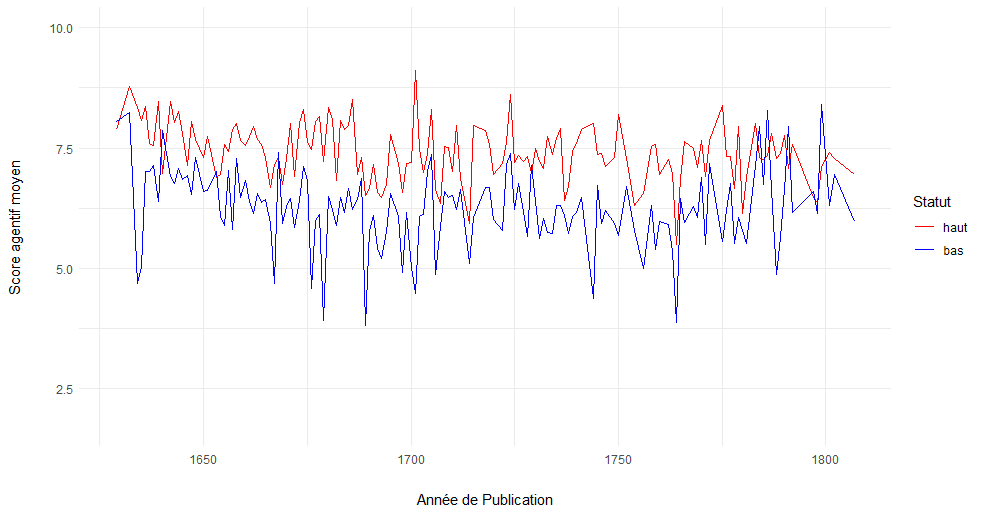
\includegraphics[width=16cm]{img/score_statut_par_annee_publication.png}
    \caption{Evolution du score agentif moyen des personnages haut et bas statut, selon l'année de publication}
    \label{score_statut_par_annee_publication}
\end{figure}

Nous avons ici réduit la période d’analyse pour ne s’intéresser qu’à l’intervalle de temps [1629-1807]. Les valeurs étant beaucoup plus espacées et extrêmes à partir de 1808, elles risquaient en effet d’influencer les résultats de façon disproportionnée. En outre, l'on précise que le score agentif analysé ci-après est celui calculé en prenant en compte la direction de corrélation prédite pour chaque métrique prise isolément (version 2 des modèles liés au statut).

De là, un modèle linéaire hiérarchique ou « à effets mixtes » incluant l'année comme intercept aléatoire permettait une première estimation de la façon dont l'effet du statut varie d'une année à l'autre. Plus précisément, en calculant la corrélation intraclasse (ICC), il apparait qu'environ 10\% de la variabilité totale du score agentif est attribuable aux différences entre les années sur la période 1629-1807.

En s’essayant à un premier regroupement des années de publication au sein de deux intervalles distincts ([1629-1699] et [1700-1807]), correspondant approximativement aux deux siècles d’analyse, et pour lesquels le nombre d’observations était globalement similaire (respectivement 450 et 414), l’on a également pu comparer les coefficients obtenus par notre modèle linéaire simple précédent (expliquant le score agentif par le statut des personnages) entre ces deux sous-périodes. L’on observe que la corrélation négative significative (p < 0.001) entre un statut « bas » et le score agentif diminue d’un intervalle à l’autre (passant de -1.163 sur la période 1629-1699 à -1.097 sur 1700-1807), ce qui est cohérent avec nos prédictions.

Malgré les limites de la présente étude, et précisément contre ces limites-mêmes concernant l’élaboration de certaines métriques individuelles, il semble donc que la conduite d’analyses successives soit justifiée (en premier lieu la détermination du caractère distinctif de notre indice). Notre indice agentif global est en effet significativement et très fortement corrélé à l’appartenance des personnages locuteurs à un « haut » statut, relativement aux personnages de  « bas » statut, et cela n'est pas simplement lié à une différence dans la longueur ou la fréquence des répliques entre ces deux types de personnages, mais bien à des marqueurs linguistiques plus fins. Il apparait même que l’on puisse déjà discerner des variations diachroniques dans cette association, bien que leur significativité, ainsi que leur corrélation avec le niveau de ressources environnant, reste encore à prouver.  
\part*{Conclusion}
\addcontentsline{toc}{part}{Conclusion}
\markboth{Conclusion}{Conclusion} 

\begin{quote}
\textit{ « Nous autres esclaves, nous sommes doués contre nos maitres \\ d’une pénétration »}
\end{quote}

Ce que Marivaux confine à une relation entre une esclave et son maitre, qui obligerait la première à un effort d’analyse des attitudes et du langage de celle qui la soumet dans la seule intention de ne pas s’y laisser prendre, et sûrement de prévenir quelques mauvais traitements, pourrait ainsi valoir beaucoup plus globalement. « Nous sommes doués \textit{comme} nos maitres d’une pénétration », voilà peut-être ce qu’aurait pu dire, à la place, le personnage esclave ou serviteur du XVIII\ieme, et dévoilant par-là l'état d'esprit de toute une époque. C’est du moins la thèse soutenue dans ce mémoire : celle d’un nivellement par le haut du degré d’agentivité individuel au cours des derniers siècles, déterminé par l’augmentation du niveau des ressources environnantes.

Pour espérer pouvoir retracer et fonder une telle évolution, il nous fallait passer par un support objectif : le langage s’est naturellement imposé comme un terrain d’analyse privilégié. 

A travers l’élaboration d’un indice linguistique d’agentivité global, il s’avère finalement possible de prédire, avec une assez grande précision, le statut des locuteurs à l’origine des répliques analysées dans une pièce donnée. Si cet indice manque encore de validité externe, il est un premier pas vers une compréhension plus fine des structures linguistiques profondes, grammaticales et syntaxiques (et outre l’utilisation de pronoms personnels à la première personne), qui pourraient bien soutenir notre discours à l’heure d’un « individualisme » exacerbé, notion intimement liée à celle d’agentivité. Et par là-même, il ouvre la porte à une étude plus approfondie des grands changements psychologiques de l’histoire humaine.

Bien entendu, si notre paradigme fait de ce degré croissant d’agentivité, ou d'individualisme tel que nous l’avons redéfini, une tendance purement mécanique, portée par l’amélioration du confort de vie, cela n’exclut pas qu’il puisse être devenu  « mal-adapté » à notre environnement actuel, au sens proprement évolutionnaire du terme. Comme mentionné dans la partie \textit{I. 2.2. Individualisme et pronoms: même méthode, nouveau raisonnement}, l’augmentation apparente des troubles neurotiques sur la période récente\footnote{\cite{twenge_age_2000}} pourrait en ce sens être interprété comme symptomatique d’une stratégie d’identification  « haut niveau » dont la quasi-permanence serait devenue sous-optimale dans nos sociétés modernes. En feignant d’ignorer ici des inégalités sociales bien entendu non négligeables, il semble en effet que tout un chacun dispose aujourd'hui, en Occident du moins, d’un niveau de ressources suffisant pour s’engager dans une interprétation particulièrement abstraite et distale de ses actions. Le moindre acte entrepris deviendrait alors le théâtre d’une délibération identitaire qu’il semble difficile de pouvoir supporter au quotidien sans risquer de se perdre, bien loin de l'agir, dans les méandres du moi. Et c’est peut-être ce que la notion d’individualisme, dans son sens péjoratif, pointe précisément du doigt. De là l’importance, également, d’études psycholinguistiques qui devraient venir compléter ces analyses dans un effort de triangularisation des données, et qui pourraient envisager y trouver, à terme, des pistes de diagnostic clinique par le biais du langage. 



% annexes
\appendix
\part*{Annexes}
\addcontentsline{toc}{part}{Annexes}
\pagestyle{myheadings}
\markboth{Annexes}{Annexes}

\section{Disponibilité des données du mémoire}\label{code}

Illustrations, code et données du mémoire disponibles sur Github à cette adresse : \url{https://github.com/CamillePerault/Agency_in_language__an_evolutionary_perspective}. 

Version \LaTeX disponible sur Github, à cette adresse \url{https://github.com/CamillePerault/redaction_Agency_in_language__an_evolutionary_perspective}.

\section{Annexe psycho-linguistique}\label{Vallacher_grille}

\begin{figure}[!ht]
    \centering
    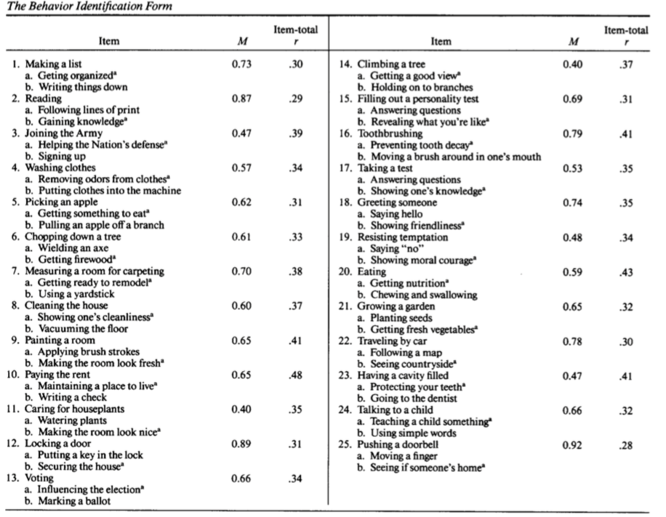
\includegraphics[width=15cm]{img/Vallacher_grille_annexe.png}
    \caption{Le « formulaire d'identification des comportements » utilisé par Vallacher (1989) afin d'estimer le degré d'agentivité de ses participants}
    \label{lm_statut}
\end{figure}

\newpage
\section{Résultats détaillés des modèles de régression}\label{result_models}

\begin{figure}[!ht]
    \centering
    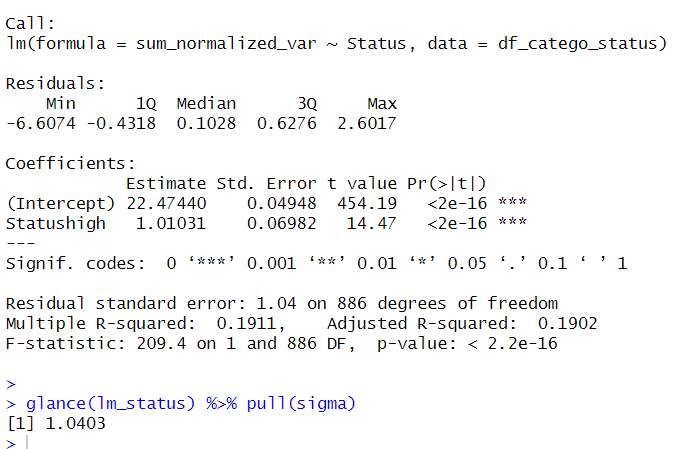
\includegraphics[width=12cm]{img/lm_statut.png}
    \caption{Résultats de la régression linéaire prédisant le score agentif par le statut - modèle 1}
    \label{lm_statut}
\end{figure}

\begin{figure}[!ht]
    \centering
    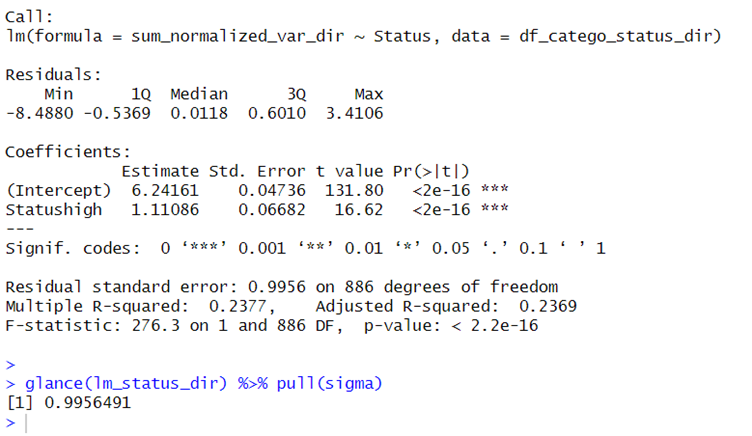
\includegraphics[width=12cm]{img/lm_statut_dir.png}
    \caption{Résultats de la régression linéaire prédisant le score agentif par le statut - modèle 2}
    \label{lm_statut_dir}
\end{figure}

\begin{figure}[!ht]
    \centering
    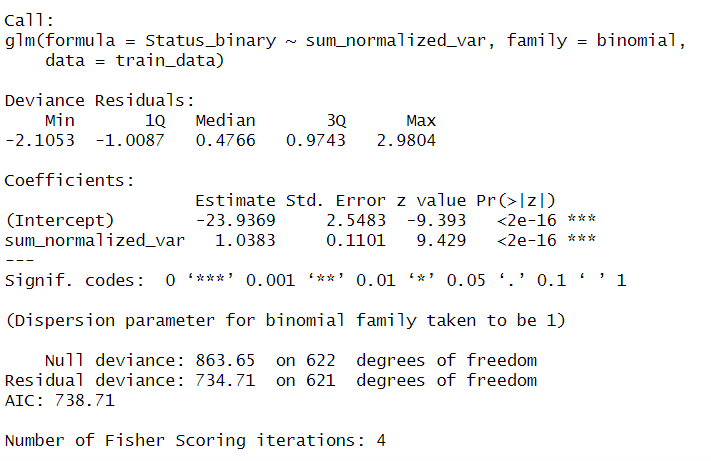
\includegraphics[width=12cm]{img/logit_statut.png}
    \caption{Résultats de la régression logistique prédisant le statut par le score agentif - modèle 1}
    \label{logit_statut}
\end{figure}

\begin{figure}[!ht]
    \centering
    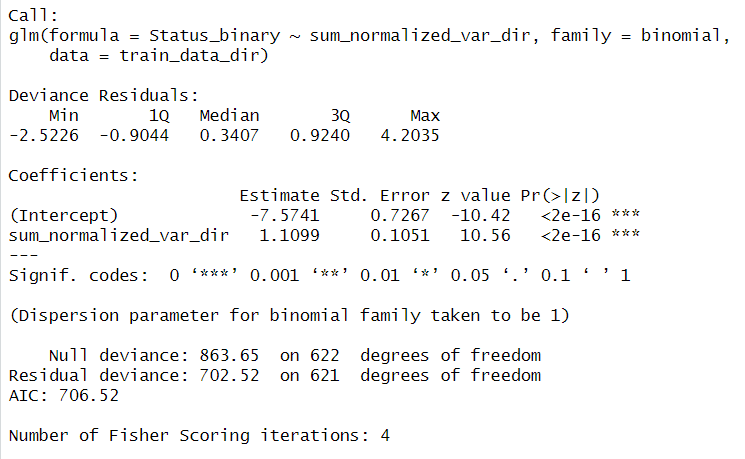
\includegraphics[width=12cm]{img/logit_statut_dir.png}
    \caption{Résultats de la régression logistique prédisant le statut par le score agentif - modèle 2}
    \label{logit_statut_dir}
\end{figure}

\begin{figure}[!ht]
    \centering
    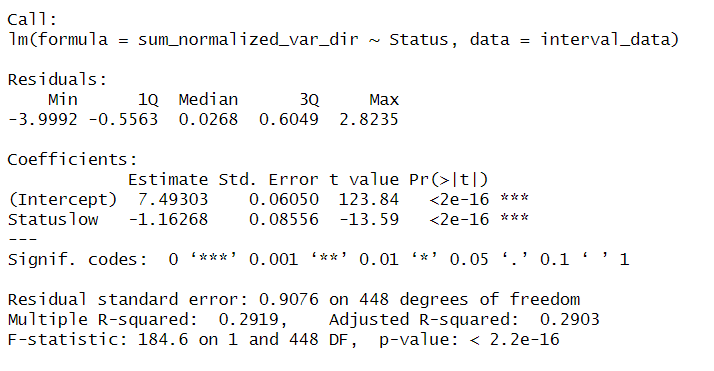
\includegraphics[width=12cm]{img/lmer1.png}
    \caption{Résultats du modèle linéaire hiérarchique intégrant l'effet de l'année de publication à la prédiction du score agentif par le statut - modèle 1}
    \label{lmer1}
\end{figure}

\begin{figure}[!ht]
    \centering
    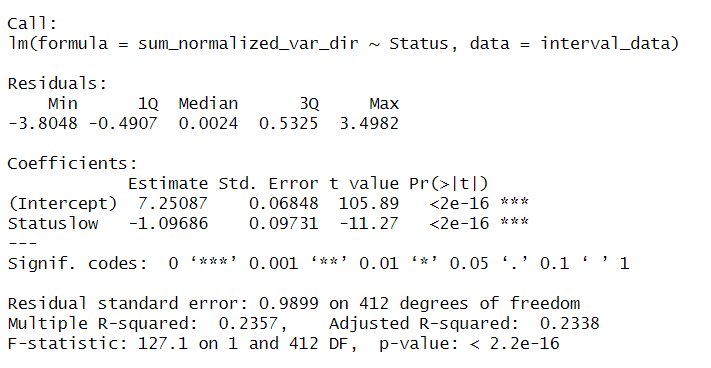
\includegraphics[width=12cm]{img/lmer2.png}
    \caption{Résultats du modèle linéaire hiérarchique intégrant l'effet de l'année de publication à la prédiction du score agentif par le statut - modèle 2}
    \label{lmer2}
\end{figure}
\backmatter

\addcontentsline{toc}{chapter}{Bibliographie}
%\nocite{*}
\printbibliography

% glossaire
%\include{back/glossaire}

% Liste des figures
\listoffigures
% table des tableaux
\listoftables


\end{document}